\Chapter{STUDENT MODELLING METHODS}\label{sec:RevLitt}

\section{ITS and EDM}
Educational Data Mining (EDM) deals with the development of methods and techniques to analyze data in an educational context. EDM uses statistical, computational, machine-learning and data mining algorithms to explore different types of educational data for resolving research questions about how students learn. Using educational softwares and also internet based education which is known as e-learning created a big data repository that provides the environment for mining educational data. Therefore using raw data coming  from educational systems and applying computational approaches can benefit learners and learning process.

Recent researches in EDM could be put in the following three categories \citep{romero2010educational} :
\begin{itemize}
\item Offline education that tries to apply statistical techniques on student's behavior and performance.
\item E-learning where web mining techniques are used to improve communication, collaboration, administration, and reporting tools.
\item Intelligent tutoring systems (ITS) that tries to adapt teaching to the needs of each particular student.
\end{itemize}

These research areas are contextually different and they require different types of data, models and techniques depending on the educational environment.

\section{Definitions and concepts}

 
\subsection{Test outcome data, Q-matrix and Skill mastery matrices}

The student test outcome data can consists in results from exams or from exercises, in the context of an e-learning environment or in paper and pencil form. We use the term \textit{item} to represent exercises, questions, or any task where the student has to apply a skilled performance to accomplish.  Student answers are evaluated and categorized as success~(1) or failure~(0).  The data represents a snapshot of the mastery of a student for a given subject matter, as we assume that the student's knowledge state has not changed from the time of anwser to the first question item to the last one.

Test data is defined as an $m \times n$ matrix, $\mathbf{R}$. It is composed of $m$~row \textit{items} and $n$~column students. Note that .  If a student successfully answers an item, the corresponding value in the results matrix is 1, otherwise it is 0.

As explained before, this results matrix $\mathbf{R}$ will be factorized into two other matrices, the skills mastery matrix and the Q-matrix.\note{Was it explained before? This is hard to understand at this point.}

The skills mastery matrix represents student skills mastery profiles. In this matrix rows are skills and columns represent examinees. A cell with the value of 1 in $\mathbf{S}_{ij}$ indicates that examinee $j$ is mastered with skill $i$ and a value of 0 shows that he does not have the related skill.

The assignment of Skills to Items is described by a Q-matrix that describes which Skill are required by each Item. In a Q-matrix rows represent Items and columns represent Latent factor (Skills). In this matrix, a cell with the value of 1 indicates the Item uses the Skill, while a 0 indicates the Skill is not involved in the item. Barnes, Bitzer, \& Vouk in \citep{barnes2005experimental} were among the early researchers to propose algorithms for automatically discovering a Q-Matrix from data.

\subsection{Partial Order Knowledge Structure(POKS)}

Skills\note{later on POKS is mentioned as a skill-less technique} are often learnt in a given order. Children learn addition, then subtraction, then multiplication, and so on. That means there should be an order for both skills and items. Based on the probabilistic models, it is possible to build such a structure form a result matrix. For example in figure \ref{fig2} four items are shown in a partial order of knowledge structure. It is required for an examinee to have skills for $i_{4}$ in order to solve $i_{3}$ and $i_{2}$. Also for solving $i_{1}$, one should have the required skills for $i_{2}$, $i_{3}$ and $i_{4}$.

\begin{figure}
\begin{footnotesize} \begin{diagram}[notextflow]    & & i_{1}:\frac{4}{\frac{12}{3}}+\frac{3}{5}=\frac{8}{5} & &   \\    & \ldTo_a & & \rdTo_b &   \\    & & & &   \\   i_{2}:\frac{4}{\frac{12}{3}}=\frac{4{\times}3}{12}=\frac{12}{12}=1 & & & & i_{3}:1+\frac{3}{5}=\frac{8}{5}  \\    & & & &   \\    & \rdTo_c & & \ldTo_d &   \\    & & i_{4}:2{\times}\frac{1}{2}=1 & &    \\  \end{diagram} \end{footnotesize}

\caption{Partial Order Structure of 4 items}


\label{fig2} 
\end{figure}


%\begin{footnotesize} \begin{diagram}[notextflow]
%   & & I1:\frac{4}{\frac{12}{3}}+\frac{3}{5}=\frac{8}{5} & &   \\
%   & \ldTo_a & & \rdTo_b &   \\
%   & & & &   \\
%  I2:\frac{4}{\frac{12}{3}}=\frac{4{*}3}{12}=\frac{12}{12}=1 & & & & I3:1+\frac{3}{5}=\frac{8}{5}  \\
%   & & & &   \\
%   & \rdTo_c & & \ldTo_d &   \\
%   & & I4:2{*}\frac{1}{2}=1 & &    \\
% \end{diagram} \end{footnotesize}


This is reflected in the results matrix $\mathbf{R}$ by closure constraints. Defining a student knowledge state as a subset of all items (i.e. a column vector in $\mathbf{R}$), then the space of valid knowledge states is closed under union and intersection according to the theory of Knowledge spaces \citep{Doignon1985}. In our study, we will relax this constraint to a closure under union, meaning that the union of any two individual knowledge states is also a valid knowledge state. This means that the constraints can be expressed as a partial order of implications among items \citep{desmarais:umuai:1996}, termed a Partial Order Knowledge Structure (POKS). A few algorithms have been defined to derive such structures from the data in $\mathbf{R}$ \citep{desmarais:umuai:1996,desmarais:2005} and the general idea of the thesis is to use this information to guide factorization algorithms.

A knowledge structure can be represented by an Oriented incidence matrix, O, or by an Adjacency matrix, A. In the oriented incidence matrix, rows are edges and columns are nodes of the graph. The value of -1 shows the start node of an edge and 1 indicates the end of an edge. Therefore for each row(edge) there is only one pair of (-1,1) and the rest of cells are 0. In adjacency matrix both rows and columns are Items and if there is a link between a pair of items(for example $i\rightarrow j$) there should be a 1 in $A_{ij}$ otherwise it is 0. Figure \ref{fig3IMAM} shows the corresponded oriented incidence matrix and adjacency matrix of the structure in figure\ref{fig2}.


\begin{figure}
\[
\begin{array}{ccccc}
\begin{array}{cc}
 & \begin{array}{cccc}
i_{1} & i_{2} & i_{3} & i_{4}\end{array}\\
\begin{array}{c}
a\\
b\\
c\\
d
\end{array} & \left(\begin{array}{cccc}
-1 & 1 & 0 & 0\\
-1 & 0 & 1 & 0\\
0 & -1 & 0 & 1\\
0 & 0 & -1 & 1
\end{array}\right)
\end{array} &  &  &  & \begin{array}{cc}
 & \begin{array}{cccc}
i_{1} & i_{2} & i_{3} & i_{4}\end{array}\\
\begin{array}{c}
i_{1}\\
i_{2}\\
i_{3}\\
i_{4}
\end{array} & \left(\begin{array}{cccc}
0 & 1 & 1 & 0\\
0 & 0 & 0 & 1\\
0 & 0 & 0 & 1\\
0 & 0 & 0 & 0
\end{array}\right)
\end{array}\\
\\
\\
O &  &  &  & A
\end{array}
\]


\caption{Oriented incidence matrix and Adjacency matrix}
\label{fig3IMAM}
\end{figure}


\section{Skills assessment and item outcome prediction techniques}

The skills assessment model we compare can be grouped into four categories: (1) the single skill Item Response Theory (IRT) approach, (2) the Knowledge Space frameworks which models a knowledge state as a set of observable items without explicit reference to skills, (3) the matrix factorization approach which decomposes the student results matrix into a Q-matrix that maps items to skills, and a skills matrix that maps skill to students, and which relies on standard matrix algebra for parameter estimation and item outcome prediction, and finally (4) the multi-skills family of DINA/DINO approaches which also refers to a Q-matrix, but incorporates slip and guess factors and relies on different parameter estimation techniques than the matrix factorization method.

Considering  these techniques more generally, we can put item outcome prediction techniques that we used in this thesis in the following categories: 
\begin{itemize}
\item Multi-Skills techniques that rely with Q-matrices to complete their prediction which are also known as skills assessment techniques. Linear techniques used in this research are Deterministic Input Noisy And/Or(DINA/DINO), NMF Conjunctive and \ac{NMF} additive
\item Single skill approaches that consider the student's ability for answering a question and they are not directly deal with a Q-matrix or set of skills. In this research we used Item Response Theory (IRT) and expected as two  techniques for item outcome prediction where they consider single skill for each student.
\item Zero skill technique that predict item outcome based on observed items. POKS is the technique that is used as a zero skill student model
\end{itemize}  
Meanwhile we defined a trivial approach as a baseline for our evaluation of the results that is called Expected Prediction approach.

However, the models reviewed here assume a static student skills state, as opposed to Knowledge Tracing model and its derivatives \cite{Koedinger2011}, for example.

The details of the specific are described below.

\section{Multi-skills techniques}

\subsection{Matrix Factorization}

Generally, matrix factorization is a method to decompose a matrix into two or more matrices. SVD and NMF are well known examples of such methods. In this research, we focus on means to improve the \ac{NMF} method.

Assume $\mathbf{R}$ is a result matrix containing student test result of ${n}$ items(questions or tests) and ${m}$ students. \ac{NMF} decompose the non-negative $\mathbf{R}$, as the product of two non-negative matrices as shown in equation\protect\eqref{eq:1}:
\begin{equation}
\mathbf{R}\approx\mathbf{Q}\mathbf{S}\label{eq:1}
\end{equation}
where $\mathbf{Q}$ and $\mathbf{S}$ are ${n}\times{k}$ and ${k}\times{m}$ respectively. $\mathbf{Q}$ is the same as Q-matrix which maps items to skills and $\mathbf{S}$ represent the skill mastery matrix that represents the mastered skills for each student. ${k}$ is called as the rank of factorization which is the same as number of latent skills. In some context there is a constraint for the number of latent skills which is : $k<nm/(n+m)$ \protect\citep{lee1999learning}

For example in the following equation , assume that we know the skills behind each item which means we know the exact Q-matrix and also we know the skills mastery as well. In this example the product of $\mathbf{Q}$ and $\mathbf{S}$ will reproduces the result matrix. Given a result matrix, we want to decompose this result matrix into the expected Q-matrix and skill mastery matrices.

\[
\begin{array}{ccccc}
\begin{array}{cc}
 & \textrm{Examinee}\\
\mathrm{\begin{sideways}Items\end{sideways}} & \left[\begin{array}{cccc}
1 & 0 & 1 & 0\\
1 & 1 & 0 & 0\\
1 & 0 & 1 & 0\\
0 & 1 & 0 & 1
\end{array}\right]
\end{array} & = & \begin{array}{cc}
 & \textrm{Skills}\\
\mathrm{\begin{sideways}Items\end{sideways}} & \left[\begin{array}{ccc}
1 & 0 & 0\\
0 & 0 & 1\\
1 & 0 & 0\\
0 & 1 & 0
\end{array}\right]
\end{array} & \times & \begin{array}{cc}
 & \textrm{Examinees}\\
\mathrm{\begin{sideways}Skills\end{sideways}} & \left[\begin{array}{cccc}
1 & 0 & 1 & 0\\
0 & 1 & 0 & 1\\
1 & 1 & 0 & 0
\end{array}\right]
\end{array}\\
\\
R &  & Q &  & S
\end{array}
\]


Many algorithms for matrix factorization search the space of solutions to equation \eqref{eq:1} by gradient descent. These algorithms can be interpreted as rescaled gradient descent, where the rescaling factor is optimally chosen to ensure convergence. Most of factorization algorithms operate iteratively in order to find the optimal factors. At each iteration of these algorithms, the new value of $\mathbf{Q}$ or $\mathbf{S}$ (for \ac{NMF}) is found by multiplying the current value by some factor that depends on the quality of the approximation in Eq. \eqref{eq:1}. It was proved that repeated iteration of the update rules is guaranteed to converge to a locally optimal factorization~\citep{seung2001algorithms}.

Besides its use for student skills assessment and for deriving a Q-matrix, matrix factorization is also a widely used technique in recommender systems where we find efforts to improve it.  \citep{koren2009matrix} shows a brief description of some of these improvements.



\subsection{Recommender systems and matrix factorization}

In the field of recommender systems, linear models have taken a central role.  Models based on matrix factorization fared particularly well in recent years.  They allow the alignment of users and votes along a few common latent factors, which was proven very efficient for predicting votes.  A culminant demonstration of the efficiency of these techniques was given in the Netflix contest~\cite{journals/sigkdd/BellK07,conf/kdd/JahrerTL10}.

The recommender systems techniques were recently applied in the field of student skills modeling~\cite{conf/its/CetintasSXH10,Toscher2010,Nguyen2011}.  The 2010 KDD Cup was held over educational data and surely helped in bringing attention of the recommender community over the task of student skills assessment.  A comparison with the widely recognized Bayesian Knowledge Tracing approach showed that it compared favorably~\cite{Nguyen2011}. Nguyen et al.\ used a multi-relational matrix and tensor-based factorization to model latent factors (skills) and the time effect to predict student success~\cite{Nguyen2011,conf/csedu/Thai-NgheDHNS11}.

The above work was conducted over dynamic student performance data.  It consists of logs of success and failures of students on exercises as they interact with a learning system environment.  These environments typically exercise the same skills over multiple problem, and often provide hints to help solve the exercises as the student faces difficulties. Obviously, learning will occur during the interaction. In fact, the same question item can be presented many times, failed one or mores time and succeeded in the end.  This is in contrast to test data where the items are presented at once without any opportunity to access learning material.  We refer to this data as static performance data.

A large body of methods have been developed for assessing student skills with static performance data (see~\cite{Desmarais2011} for a review).  For the vast majority, these methods are either non linear models or general linear models (for eg.~logistic regression). The most widely used one is Item Response Theory (IRT)~\cite{birnbaum:1968}.  Although it and it dates back to almost 50~years, it remains one of the most prominant and an active field of research in psychometrics (for eg.~\cite{bakerKim2004}).

\subsection{Similarity with recommender systems and assumptions}

Equation~(\ref{eq:nmf}) is analoguous to the decomposition of the (\textit{item} $\times$ \textit{user}) votes matrix into two smaller matrices: the (\textit{item} $\times$ \textit{preference}) and (\textit{preference} $\times$ \textit{user}) matrices.  However, the the votes matrix is typically sparse and different means have been developed to accomodate matrix factorization techniques with sparse matrices, and to compensate for predictions based on highly uneven number of votes in columns and rows that tend to negatively affect the predictive performance of algorithms.



\subsection{Non-Negative Matrix Factorization(\ac{NMF})}

\ac{NMF} is a factorization technique that decompose a matrix into two matrices. The prominent characteristic of \ac{NMF} is the non-negative constraint on the decomposed elements. \ac{NMF} imposes this constraint and consequently all those values in the decomposed elements are non-negative.

The clear point of this decomposition is that there can be different solutions. Although the constraint of non-negative elements eliminate some solutions but still there may be different solutions for this factorization

It is important to emphasize that there are many solutions to $\mathbf{R}\approx\mathbf{Q}\mathbf{S}$. Different algorithms may lead to different solutions. Indeed, many \ac{NMF} algorithms have been developed in the last decade and they can yield different solutions. We refer the reader to \citep{Berry2007} for a more thorough and recent review of this technique which has gained strong adoption in many different fields. 

Gradient decent is one of the best known approaches for implementing  \ac{NMF}.  If $k$ is less than the minimum of $m$ and $n$, finding the exact $\mathbf{Q}$ and $\mathbf{S}$ matrices which satisfy $\mathbf{R}=\mathbf{Q}\mathbf{S}$ can entail a loss of information. Therefore this algorithm tries to get the best estimation for $\mathbf{Q}$ and $\mathbf{S}$ to make $\mathbf{R}\approx\mathbf{Q}\mathbf{S}$ more accurate. Based on the definition of gradient descent method, a cost function should be defined to quantify the quality of the approximation. This cost function can be a measure of distance between two non-negative matrices $\mathbf{R}$ and $\mathbf{Q}\mathbf{S}$. It  can be the Euclidean distance between these two matrices as shown in equation \eqref{eq:3} where $\mathbf{Q}_{i}$ is a row vector of $\mathbf{Q}$ and $\mathbf{S}_{j}$ is a column vector of $\mathbf{S}$ and $\mathbf{R}_{ij}$ is cell $(i,j)$ of $\mathbf{R}$.

\begin{equation}
\left\Vert \mathbf{R}-\mathbf{Q}\mathbf{S}\right\Vert ^{2}=\sum_{{\scriptscriptstyle ij}}(\mathbf{R}_{ij}-\mathbf{Q}_{i}\mathbf{S}_{j})^2\label{eq:3}
\end{equation}


  
Another cost function  is based on the Kullback-Leibler divergence, which measures the divergence between $\mathbf{R}$ and $\mathbf{Q}\mathbf{S}$ as shown in equation \eqref{eq:4}. 
\begin{equation}
D(\mathbf{R}||\mathbf{Q}\mathbf{S})=\sum_{{\scriptscriptstyle ij}}(\mathbf{R}_{ij}log\frac{\mathbf{R}_{ij}}{\mathbf{Q}_{i}\mathbf{S}_{j}}-\mathbf{R}_{ij}+\mathbf{Q}_{i}\mathbf{S}_{j})\label{eq:4}
\end{equation}

In both approaches, the goal is
to minimize the cost function where they are lower bounded by zero and it happens only if $\mathbf{R}=\mathbf{Q}\mathbf{S}$ \citep{seung2001algorithms}. For simplicity we just consider the cost function based on the Euclidean
distance.

The gradient descent algorithm used to minimize the error is iterative and in each iteration we expect a new estimation of the factorization. We will refer to the estimated Q-matrix{ as} $\hat{\mathbf{Q}}$ and{ the} estimated Skill mastery matrix{ as} $\hat{\mathbf{S}}$.  The iterative gradient descent algorithm should change $\mathbf{Q}$ and $\mathbf{S}$ to minimize the cost function. This change should be done by an update rule. Lee and Seung \citep{seung2001algorithms} found the following update rule in equation \eqref{eq:5}. These update rules in equation \eqref{eq:5} guarantee that the Euclidean distance $\left\Vert \mathbf{R}-\mathbf{Q}\mathbf{S}\right\Vert $ is non increasing during the iteration of the algorithm.

\begin{equation}
\begin{aligned}\hat{\mathbf{S}}\leftarrow\hat{\mathbf{S}}\frac{(\mathbf{\hat{Q}}^{T}\mathbf{R})}{(\hat{\mathbf{Q}}^{T}\mathbf{\hat{Q}}\hat{\mathbf{S}})}\end{aligned}
\hspace{20mm}\begin{aligned} & \mathbf{\hat{Q}}\leftarrow\mathbf{\hat{Q}}\frac{(\mathbf{R}\mathbf{\hat{\mathbf{S}}}^{T})}{(\mathbf{\hat{Q}}\mathbf{\hat{\mathbf{S}}}\mathbf{\hat{\mathbf{S}}}^{T})}\end{aligned}
\label{eq:5}
\end{equation}


The initial value for Q and S are usually random but they can be adjusted to a specific method of \ac{NMF} library to find the best seeding point.


\subsection{Types of Q-matrix}

There are three models for the Q-matrix which are useful based on the context of the problem domain. The most important one is the conjunctive model of the Q-matrix which is the standard interpretation of the Q-matrix. In figure \ref{fig1} an example of conjunctive model of Q-matrix is shown. Examinee $e_{1}$ answered item $i_{1}$ and item $i_{4}$ because he has mastered in the required skills but although he has skill $s_{1}$ he couldn't answer item $i_{3}$ which requires skill $s_{2}$ as well.

Barnes \citep{Barnes2005} proposed equation \ref{eq:6} for this model where the operator $\neg$ is the boolean negation that maps 0 values to 1 and other values to 0. In this way, if an examinee that mastered all required skills for an item, he will get 1 in the result matrix otherwise he will get a 0 value, even if the required skills are partially mastered.

In fact if we apply a boolean negation function to both sides of the equation \ref{eq:6}, we will see that the $\neg\mathbf{R}$ matrix is a product of two matrices, $\mathbf{Q}$ and $\neg\mathbf{S}$

\begin{equation}
\mathbf{R}=\neg\left(\mathbf{Q}\left(\neg\mathbf{S}\right)\right)\label{eq:6}
\end{equation}


\begin{figure}
\begin{footnotesize} 
\[
\begin{array}{ccc}
\begin{array}{cc}
 & \textrm{Examinee}\\
 & \begin{array}{cccc}
e_{1} & e_{2} & e_{3} & e_{4}\end{array}\\
\mathrm{\begin{sideways}Items\end{sideways}}\begin{array}{c}
i_{1}\\
i_{2}\\
i_{3}\\
i_{4}
\end{array} & \left[\begin{array}{cccc}
1 & 0 & 1 & 0\\
0 & 1 & 0 & 0\\
0 & 0 & 1 & 0\\
1 & 0 & 0 & 0
\end{array}\right]
\end{array} & \begin{array}{cc}
 & \textrm{Skills}\\
 & \begin{array}{ccc}
s_{1} & s_{2} & s_{3}\end{array}\\
\mathrm{\begin{sideways}Items\end{sideways}}\begin{array}{c}
i_{1}\\
i_{2}\\
i_{3}\\
i_{4}
\end{array} & \left[\begin{array}{ccc}
1 & 0 & 0\\
0 & 1 & 1\\
1 & 1 & 0\\
1 & 0 & 1
\end{array}\right]
\end{array} & \begin{array}{cc}
 & \textrm{Examinees}\\
 & \begin{array}{cccc}
e_{1} & e_{2} & e_{3} & e_{4}\end{array}\\
\mathrm{\begin{sideways}Skills\end{sideways}}\begin{array}{c}
s_{1}\\
s_{2}\\
s_{3}
\end{array} & \left[\begin{array}{cccc}
1 & 0 & 1 & 0\\
0 & 1 & 1 & 1\\
1 & 1 & 0 & 0
\end{array}\right]
\end{array}\\
\\
R & Q & S
\end{array}
\]
 \end{footnotesize} \caption{An example for Conjunctive model of Q-matrix}


\label{fig1} 
\end{figure}


In this research we focus on the conjunctive model of Q-matrix but there are two other types of Q-matrices: disjunctive and compensatory. In the disjunctive model, there is a disjunction between skills of an item. At least one of the required skills should be mastered in order to have a success in answering the related item.

Compensatory or additive model of skills is an interpretation of a Q-matrix where skills have weights to yield a success for that item. For example, considering an item requires two skills $a$ and $b$ with the same weight each. Then each skill will contribute equally to yield a success of the item. In the compensatory model of Q-matrix, each skills increase the chance of success based on its weight.

\subsection{Deterministic Input Noisy And/Or (DIAN/DINO)}

\note{This one differs because it assumes an existing Q-matrix.}

The other skills assessment model we consider are based on what is referred to as Deterministic Input Noisy And/Or (DINO/DINA) \cite{junker2001cognitive}.  They also rely on a Q-matrix. The DINA model (Deterministic Input Noisy And) corresponds to the conjunctive model whereas the DINO (Deterministic Input Noisy Or) corresponds to the disjunctive one, where the mastery of a single skill is sufficient to succeed an item.  The acronyms makes reference to the AND/OR gates terminology.

These models predict item outcome based on three parameters: the slip and guess factors of items, and the different ``gate'' function between the student's ability and the required skills.  The gate functions are equivalent to the conjunctive and disjunctive vector product logic described for the matrix factorization above.  In the DINA case, if all required skills are mastered, the result is~1, and 0~otherwise. Slip and guess parameters are values that generally vary on a~$[0,0.2]$ scale. In the DINO case, mastery of any skills is sufficient to output~1.  Assuming~$\xi$ is the output of the corresponding DINA or DINO model and~$s_j$ and~$g_j$ are the slip and guess factors, the probability of a successful outcome to item~$X_{ij}$ is:
\begin{equation}
 P(X_{ij} \!=\! 1 \; | \; \xi_{ij}) \,=\, (1-s_j)^{\xi_{ij}} g_j^{1-\xi_{ij}}
\label{DinoEQ}
\end{equation}

The DINO model is analog to the DINA model, except that mastery follows the disjunctive
framework and therefore~$\xi_{ij}=1$ if \textit{any} of the skills required by item~$j$ are
mastered by student~$i$.

A few methods have been developed to estimate the slip and guess parameters from data and we use the one implemented in the R~CDM package \citep{Robitzsch2012}.

\subsection{Alternate Least-square Factorization (ALS)}
\label{ALS-Def}

The {Alternate Least-Square Factorization (ALS)} method is defined in \cite{Desmarais2013aied} which is also a factorization method. Starting with the results matrix ~$\mathbf{R}$ and an initial Q-matrix, $\mathbf{Q}_0$, a least-squares estimate of the skills matrix ~$\mathbf{\hat{S}}_0$ can be obtained by:

\[
  \mathbf{\hat{S}}_0 = (\mathbf{Q}_0^{\mathrm{T}}  \, \mathbf{Q}_0)^{-1} \, \mathbf{Q}_0^{\mathrm{T}} \, \mathbf{R} \label{eq:shat}
\]

The initial matrix~$\mathbf{{Q}}_0$ is the expert defined Q-matrix. Then, a new estimate of the Q-matrix, $\mathbf{\hat{Q}}_1$, is again obtained by the least-squares estimate:
\[
  \mathbf{\hat{Q}}_1 = \mathbf{R} \, \mathbf{\hat{S}}_0^{\mathrm{T}} \, (\mathbf{\hat{S}}_0 \, \mathbf{\hat{S}}_0^{\mathrm{T}})^{-1} \label{eq:qhat}
\]
And so on for estimating~$\mathbf{\hat{S}}_1$, ~$\mathbf{\hat{Q}}_2$, ... Alternating between equations~(\ref{eq:shat}) and~(\ref{eq:qhat}) yields progressive refinements of the matrices~$\mathbf{\hat{Q}}_i$ and ~$\mathbf{\hat{S}}_i$ that more closely approximate~$\mathbf{R}$ in equation~(\ref{eq:nmf}).  The convergence is based on a predefined delta between iterations. In our experiments we consider delta as $0.001$ that makes the algorithm to converge after few iterations .This performance makes the technique many times more efficient than factorizations that rely on gradient descent, for example.

The ALS factorization is \textit{compensatory} in the above description.  A \textit{conjunctive} version can be obtained by inverting the values of the $\mathbf{R}$~matrix~\cite{Desmarais2012b}.  

It is worth mentioning that, by starting with non negative matrices ~$\mathbf{{Q}}_0$ and ~$\mathbf{R}$, the convergence process will generally end with positive values for both matrices ~$\mathbf{\hat{Q}}_i$ and ~$\mathbf{\hat{S}}_i$. The vast majority of values obtained are between 0.5 and 1.5 if both the results matrix and the initial Q-matrix have {0,1} values. Also regularization terms could be used in the implementation of the algorithm to force non-negative or integer values.

Note that ~$(\mathbf{Q}_0^{\mathrm{T}} \, \mathbf{Q}_0)$ or ~$(\mathbf{\hat{S}}_0 \,
\mathbf{\hat{S}}_0^{\mathrm{T}})_0$ may not be invertable, for example in the case where the
matrix~$\mathbf{Q}_0$ is not column full-rank, or the matrix~$\mathbf{S}_0$ is not row full-rank.  This is
resolved by adding a very small Gaussian noise before attempting the inverse.  Ensuring the choice of a
relatively insignificant noise does not affect the end result for our purpose. 


\subsection{Other Techniques to Derive Q-matrices from Data}

\note{The derivation of a Q-matrix from data is a prerequesite for some models whereas it sometimes is a given for others.  This should probably be explained beforehand.  It also makes a good argument for the work on the induction of a Q-matrix from data since, without it, performance cannot be assessed for these models.}

Cen et al. \citep{Cen2005,Cen2006} have used Learning FactorAnalysis technique(LFA) technique to improve the initially hand built Q-matrix which maps fine-grained skills to questions. They used log data which is based on the fact that the knowledge state of student dynamically changes over time as the student learns. In the case of static data of student knowledge, Barnes \citep{Barnes06} developed a method for this mapping which works based on a measure of the fit of a potential Q-matrix to the data. It was shown to be successful as well as Principle Component Analysis for skill clustering analysis.

In the experiments of Winters et al. \citep{Winters05}, different standard clustering techniques for finding the Q-matrix were applied on different types of datasets. Some datasets from SAT topics such as Mathematics, Biology and French, to computer science exams, and to different trivia topics were tested with the clustering techniques. It was shown that those techniques were successful at separating items that belongs to totally different topics, for example mathematics and french. For topics without any skill behind them(essentially they are facts and the only skill required is to memorize them), topic separation was less successful.


\section{Single skill approaches \note{should probably be earlier since it is easier to explain}}


\subsection{IRT}

The \textbf{IRT family} is based on a logistic regression framework. It models a single latent skill (although variants exists for modeling multiple skills) \cite{bakerKim2004}.  Each item has a difficulty and a discrimination parameter.

IRT assumes the probability of success to an item~$X_j$ is a function of a single ability factor~$\theta$: 
\[P(X_j\!=\!1\;|\;\theta) = \frac{1}{1+e^{-a_j(\theta-b_j)}}\]
In the two parameter form above, referred to as IRT-2pl, parameter~$a$ represents the item discrimination and parameter~$b$ represents the item difficulty.  

The ability of a single student, $\theta_i$ is estimated by maximizing the likelihood of the observed response outcomes probabilities:
\[ P(X_1, X_2, ..., X_j, \theta_i) = \prod_j P(X_j|\theta_i) \]
This corresponds to the usual logistic regression procedure.

The specific IRT skills assessment version is the Rash model, for which the discrimination parameter~$a$ is fixed to~$1$.  Fixing this parameter reduces over fitting, as the discrimination can sometimes take unrealistically large values. Note however that we do generate synthetic data from the more general IRT-2pl model to make this data more realistic.


\subsection{Baseline expected value}

As a baseline model, we use the expected value of success to an item~$i$ by student~$j$, as defined by a product of odds:
\[ O(X_{ij}) =  O(X_i) O(S_j) \]
where $O(X_i)$ are the odds of success to item~$i$ and $O(S_j)$ are the odds of success of student~$j$.  Both odds can be estimated from a sample.  Recall that the transformation of odds to probability is $P(X) = 1/(1+O(X))$, and conversely $O(X) = P(X)/(1 - P(X))$. probabilities are estimated using the Laplace correction: $P(X) = (f(x\!=\!1) + 1) / (f(x\!=\!1) + f(x\!=\!0) + 2)$


\section{Zero skill technique}

\note{Needs an introduction.  }

\subsection{Knowledge Spaces and Partial Order Knowledge Structures (POKS)}

The {knowledge spaces} approach models a knowledge domain as a set of observable items. An individual's knowledge state is represented as a subset of these items.  The ``knowledge space'' determines the valid subsets of items. There are no explicit latent skills, but skills assessment can be obtained from the estimated item outcomes given a Q-matrix.

The model adopted to assess knowledge is POKS (Partial Order Knowledge Structures), which is a more constrained version of Knowledge Spaces theory \cite{desmarais:umuai:1995}.  POKS assumes that items are learned in a strict partial order.  It uses this order to infer that the success to hard items increases the probability of success to easier ones, or conversely, that the failure to easy items decreases the chances of success to harder ones.

The structure of the partial order of items is obtained from a statistical hypothesis test that reckons the existence of a link between two items, say $A \rightarrow B$, on the basis of two Binomial statistical tests $P(B|A) > \alpha_1$ and $P(\neg A|\neg B) > \alpha_1$ and under a predetermined alpha error ($\alpha < \alpha_2)$.  The values of $\alpha_1 = .85$ and $\alpha_2 = .10$ are chosen in this study across all experiments.

A student knowledge state is represented as a vector of probabilities, one per item.  Probabilities are updated under a Naive Bayes assumption as simple posterior probabilities given observed items.





\section{Recent improvements}


Curriculum design can be a complex task and an expert blind spots in designing curricula is possible. It is desirable to have an alternative to human sequenced curricula. To do so, there should be a model designed for this purpose which maps latent factors (simply referred to as skills, concepts or facts in the field of ITS) to items (simply referred to as questions) \citep{Tatsuoka1983,Tatsuoka2009}. Figure \ref{QItemInt} shows an example of this mapping which is named  Q-matrix.  Figure \ref{ItemInt} shows 4 items and each item requires different skills (or combination of skills) to be successfully answered. Assuming 3 skills such as fraction multiplication ($s_{1}$), fraction addition ($s_{2}$) and fraction reduction($s_{3}$), these questions can be mapped to skills like the Q-matrix represented in figure \protect\ref{QInt}. Such a mapping is desirable and very important in student modelling; because optimal order of problems(sequence of repetition and presentation) can be determined by this model since it allows prediction of which item(question or problem) will cause learning of skills that transfer to the other items most efficiently. It can also be used to assess student knowledge of each concept, and to personalize the tutoring process according to what the student knows or does not know.  For example, Heffernan et al. in \citep{feng2009using} have developed an intelligent tutoring system (the ASSISTment system) that relies on fine grain skills mapped to items.
  

\begin{footnotesize}
\begin{figure}[ht]
\centering

\subfigure[Items with different skills]{
   $\begin{array}{cc}
i_{1} & \frac{4}{\frac{12}{3}}+\frac{3}{5}=\frac{8}{5}\\
 &  \\
i_{2} & \frac{4}{\frac{12}{3}}=\frac{4{\times}3}{12}=\frac{12}{12}=1\\
 &  \\
i_{3} & 1+\frac{3}{5}=\frac{8}{5}\\
 &  \\
i_{4} & 2{\times}\frac{1}{2}=1\\
&
\end{array}$
\label{ItemInt}
}
\quad
 \subfigure[Q-matrix]{

$\begin{array}{c}
\begin{array}{cc}
 & \textrm{Skills}\\
 & \begin{array}{ccc}
s_{1} & s_{2} & s_{3}\end{array}\\
\mathrm{\begin{sideways}Items\end{sideways}}\begin{array}{c}
i_{1}\\
i_{2}\\
i_{3}\\
i_{4}
\end{array} & \left[\begin{array}{ccc}
1 & 1 & 1\\
1 & 0 & 1\\
0 & 1 & 1\\
1 & 0 & 1
\end{array}\right]
\end{array}\\
\\
\\

\end{array}$
\label{QInt}
}
\caption{Items and Q-matrix}\label{QItemInt}
\end{figure}
\end{footnotesize}


Different techniques and methods in the field of data mining were used to derive a Q-matrix. Matrix factorization is one of the most important one in this area. Matrix factorization is a method to decompose a matrix into two or more matrices. It is an important technique in different fields such as skill modelling, bioinformatics, and vision, to name but a few. It has achieved great results in each of these fields. For skills assessment, Nguyen et al. \citep{Nguyen2011} have shown that the approach can lead to assessments that reach prediction accuracies comparable and even better than well established techniques such as Bayesian Knowledge Tracing \citep{corbett:umuai:1995}. Matrix factorization can also lead to better means for mapping which skills can explain the success to specific items.

It has been shown that this mapping can be derived by Matrix Factorization techniques \citep{desmarais2011conditions,desmarais2012item} on a test result data with different topic such as history, biology, math and french. Considering a single skill for each topic, the derived Q-matrix can represent a single skill per item mapping. Dealing with Q-matrices that success or failure of an item depends on more than one skill requires more complicated interpretation. 
A general contribution for such a problem is identifying a optimize number of skills for a set of items. It has been reported in \citep{lee1999learning} that number of skills should conform to : $r < nm/(n+m)$ where $r$, $n$ and $m$ is the number of skills, items and students respectively. Finding the best number of skills which counts all the essential and useful skills is always desired. The other part of this thesis is to define approaches to find the optimum number of skills for creating a Q-matrix. Finally, the last step for improving the quality of an expert defined Q-matrix is to verify and refine its accuracy  based on some approaches that we will discuss in next chapters.



The rest of this chapter presents some researches that are related to the main contribution of this thesis. The general perspective of section \ref{ITS2012} is to find a way for deriving the Q-matrix from data, along with a Skills mastery matrix. We aim to find a method to derive these matrices for different types of Q-matrices. This should be a valuable and challenging task. Finding the number of latent skills (i.e. the common dimension between matrices $\mathbf{Q}$ and~$\mathbf{S}$) is another important task that is described in section \ref{ITS2012} . Finally, in section \ref{edm2014} we will introduce methods to validate tasks to skills mapping which is also applicable for the refinement of a Q-matrix.

The following sections will describe these completed researches.


\section{NMF on single skill and multi-skill conjunctive Q-matrix}
\label{ITS2012}

A few studies have shown that a mapping of skills to items can, indeed, be derived from data \citep{delafayette2006educational,desmarais2011conditions}. Winters et al. showed that different data mining techniques can extract item topics, one of which is matrix factorization \citep{delafayette2006educational}. They showed that NMF works very well for simulated data, but the technique\textquoteright{}s performance with real data was degraded. Their study showed that only highly distinct topics such as mathematics and French can yield a perfect mapping. Biology and history were the other topics in this research which were named as general topics. Clustering of these topics was not accurate because they are factual knowledge and they are not comparable with some topics like mathematics.

This study was later corroborated by Desmarais \citep{desmarais2011conditions} who also used simulated data to show that the low discrimination power of some topics might be explained by their lower weight in terms of skill factors, when compared to other factors such as item difficulty and student ability.

The factorization methods in the studies mentioned above rely on the standard matrix operators which was in formula \ref{eq:1} and therefore can be considered as compensatory models of Q-matrix which was explained in the previous chapter. Actually, in these study all items rely on one skill and there was not a combination of skills for any item, thus the simple model of factorization will work. 

To follow up the on previous studies \citep{Barnes2005,desmarais2011conditions,Winters07} we can apply NMF technique to equation \ref{eq:6}. The goal of this task is to determine if NMF can successfully derive a conjunctive model of Q-matrix , where skills do not add up to increase the chances of success to an item, but instead are necessary conditions.


%\subsection{Simulated data}

%To validate the technique, we rely on simulated data. Although it lacks the external validity of real data, it remains the most reliable means of obtaining test results data for which the underlying, latent skills structure is perfectly known. Therefore, assessing the technique over simulated data is a reasonable first step to establish the validity the approach under controlled conditions. Further studies with real data will be necessary, granted the results of the existing study warrants such work.

%Whilst the underlying model and methodology of the simulated data are shown to make substantial performance of student skills assessment (see \citep{Desmarais2010a} for eg.), we describe in some details this methodology. 

%A first step to obtain data of simulated examinee test results is to define a Q-matrix composed of $j$ skills and $k$ items. We chose to define a Q-matrix that spans all possible combinations of 6 skills with a maximum of two skills per item, and at least one skill per item. A total of 21 items spans this space of combinations. This matrix is shown in Figure \ref{figqmatrixandResutM}. Items 1 to 15 are two-skills and items 16 to 21 are single-skill. 

%\begin{figure}[ht]
%\centering

%\subfigure[Q-matrix of 6 skills and for which 21 items are spanning the full set of 1 and 2 skill combinations]{
 %  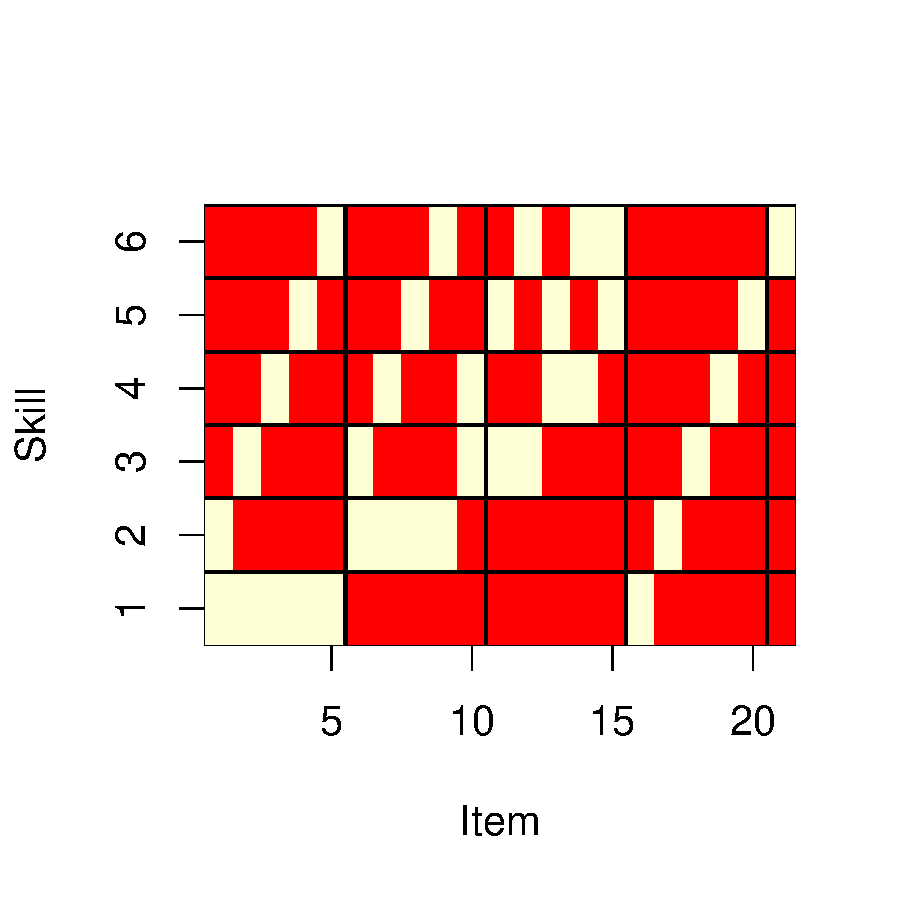
\includegraphics[scale =0.5] {ExpectedQ}\label{PerfectQ}
 %}\quad
 %\subfigure[Simulated data example of 100 examinees with parameters: slip: 0.1, guess: 0.2, skills difficulties: ($0.17$, $0.30$, $0.43$, $0.57$, $0.70$, $0.83$)]{
%   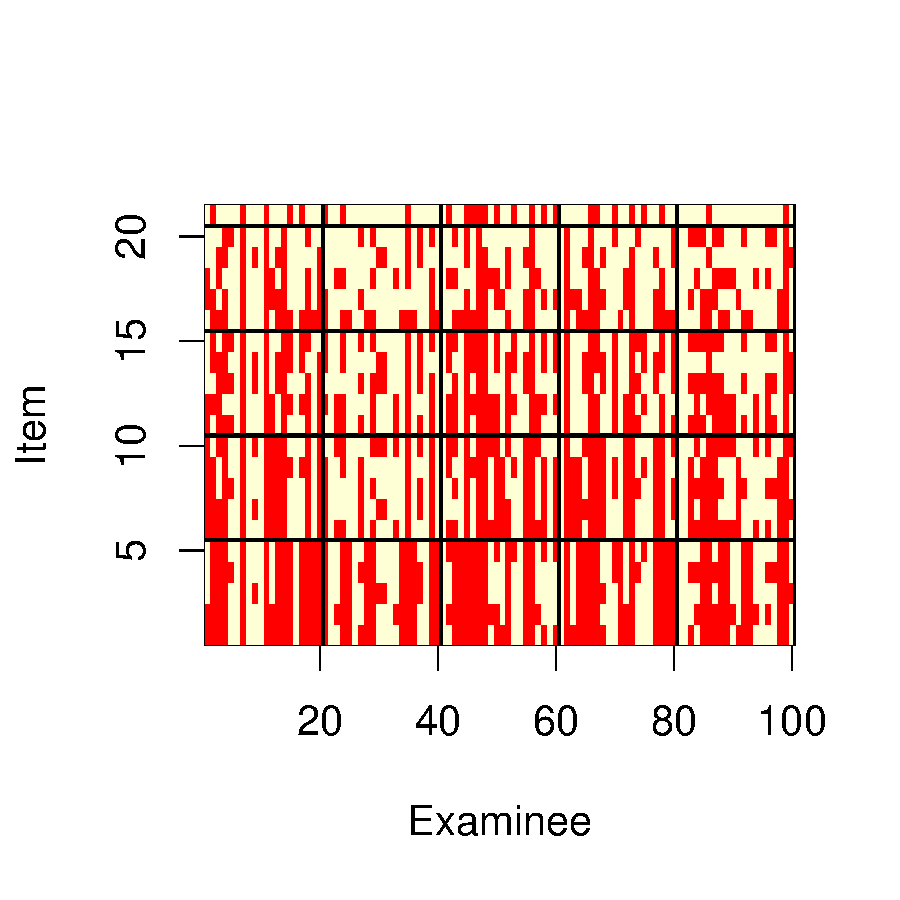
\includegraphics[scale =0.5] {ResultM}
 %}
%\caption{Q-matrix and an example of simulated data with this matrix.  Bright pixels represent 1's and dark red ones represent 0's.}
%\label{figqmatrixandResutM}
%\end{figure}


%We will consider that skills have a difficulty level. That difficulty will transfer to items that have this skill. The difficulty of the two-skills items will further increase by the fact that they require the conjunction of their skills. We do not assign an item difficulty since this is already reflected by skill difficulties.

%Examinees need to be assigned ability levels. The ability is, in fact, reflected by the set of skills mastered. Ability variance will therefore show up as the variance in number of skills across examinees, and the assigned ability level will increase this variance over the variance resulting from skill difficulty.

%Finally, two more parameters are used in the simulated the data, namely the $\mathit{slip}$ and $\mathit{guess}$ factors. These factors are set as constant values across items. They are essentially noise factors and the greater they are, the more difficult is the task of inducing the Q-matrix from data.

%Given the above framework, the process of generating simulated examinee data follows the following steps:
%\begin{enumerate}
%\item Assign a difficulty level to each skill.
%\item Generate a random set of hypothetical examinee skills vectors based on the difficulty of each skill and the examinee\textquoteright{}s ability level. Skill difficulty and examinee ability are each expressed as a random normal variable. The probability density function of their sum provides the probability of mastery of the skill for the corresponding examinee. The skill vector is a sampling in \{0, 1\} based on each skill probability of mastery. 
%\item Generate simulated data based on equation \ref{eq:6} without taking into account the $\mathit{slip}$ and $\mathit{guess}$ parameters. This is referred to as the $ideal$ response pattern.
%\item Randomly change the values of the generated data based on the $\mathit{slip}$ and $\mathit{guess}$ parameters. For example, with values of 0.1 and 0.2 respectively, this will result in approximately $10\%$ of the succeeded items to become failed, and $20\%$ of the failed items to become succeeded.
%\end{enumerate}
%The first two steps of this process are based on additive gaussian factors and follow a similar methodology to \citep{desmarais2011conditions}.

%A sample of the results matrix is given in figure\ref{figqmatrixandResutM}. Examinee ability shows up as vertical patterns, whereas skills difficulty creates horizontal patterns. As expected, the mean success rate of the 2-skills items 1 to 15 is lower than the single skill items 16 to 21.



\subsection{Simulation methodology}


The assessment of the NMF performance to infer a Q-matrix from simulated test data such as figure \ref{figqmatrixandResutM}'s is conducted by comparing the predefined Q-matrix, $\mathbf{Q}$, as shown in figure \ref{figqmatrixandResutM}, with the $\hat{\mathbf{Q}}$ matrix obtained in the NMF of equation \ref{eq:6}.

As mentioned above, the negation operator is applied over the simulated test data and the NMF algorithm is carried over this data. We used the R NMF package \citep{Gaujoux2010} and the Brunet NMF algorithm.

We defined a specific method for the quantitative comparison of the matrix $\hat{\mathbf{Q}}$ with $\mathbf{Q}$. First, the $\hat{\mathbf{Q}}$ matrix contains numerical values on a continuous scale. To simplify the comparison with matrix $\mathbf{Q}$, which is composed of \{0, 1\} values, we discretize the numerical values of $\hat{\mathbf{Q}}$ by applying a clustering algorithm to each item in $\hat{\mathbf{Q}}$, forcing two clusters, one for 0\textquoteright{}s and one for 1\textquoteright{}s. For example, item 1 in the NMF inferred matrix of figure \ref{ClusteringResults}  (which we explain later) corresponds to a vector of six numerical values, say \{1.6, 1.7, 0.0015, 0.0022, 0.0022, 0.0018\}. This vector clearly cluster into the \{1, 1, 0, 0, 0, 0\} vector of item 1 in figure \ref{ClusteringResults}. The K-means algorithm is used for the clustering process of each item and we use the kmeans routine provided in R (version 2.13.1).

Then, to determine which skill vector (column) of the $\hat{\mathbf{Q}}$ matrix corresponds to the skill vector of the $\mathbf{Q}$ matrix, a correlation matrix is computed and the highest correlation of each column vector $\hat{\mathbf{Q}}$ is in turn matched with the corresponding unmatched column in $\mathbf{Q}$.

We will use visual representations of the raw and the \textquotedblleft{}discretized\textquotedblright{} (clustered) $\hat{\mathbf{Q}}$ matrix to provide an intuitive view of the results, as well as a quantitative measures of the fit corresponding to the average of the correlations between the matched skills vectors $\hat{\mathbf{Q}}$ and $\mathbf{Q}$.


\subsection{Results}


In order for the mean and variance of the simulated data to reflect realistic values of test data, the skill difficulty and examinee ability parameters are adjusted such that the average success rate is close to 60\%. Examinee ability is combined with the skill difficulty vectors to create a probability matrix of the same dimensions as $\mathbf{S}$, from which $\mathbf{S}$ is obtained.


\begin{figure}[!h]
\centering

\subfigure[Matrix $\hat{\mathbf{Q}}$ without slip and guess factors ($r=1$)]{
   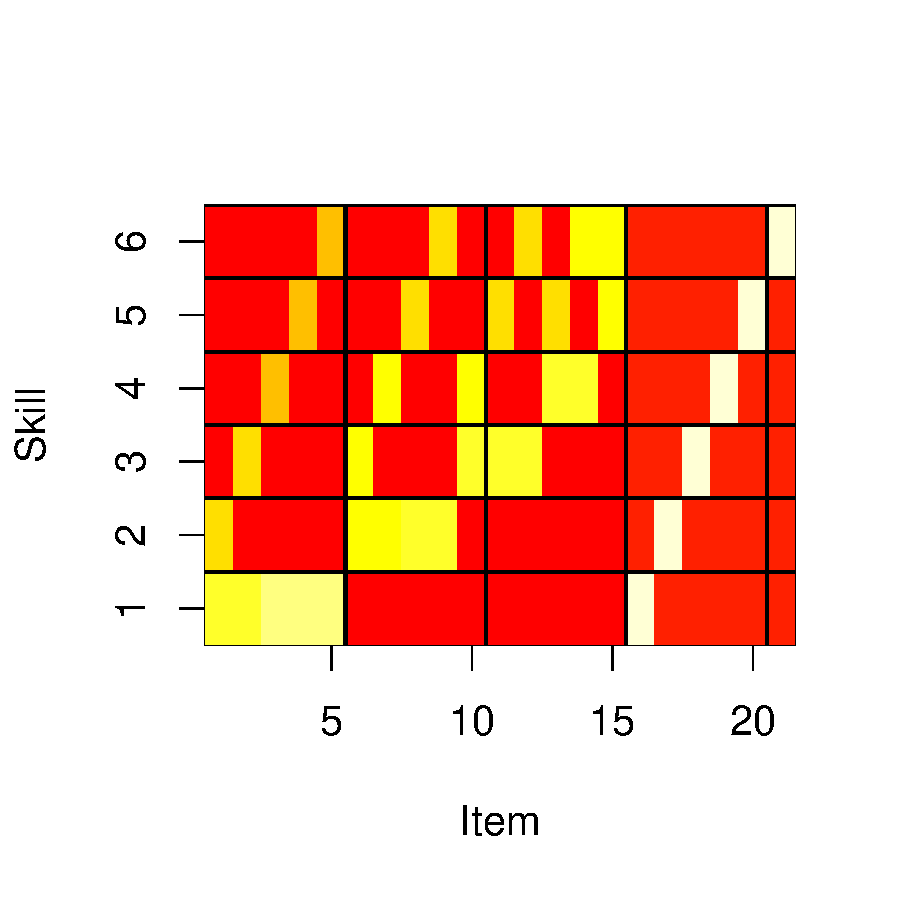
\includegraphics[scale =0.5] {NONnoiseQ}\label{NonnoisyQ}
 }\quad
 \subfigure[Discretized $\hat{\mathbf{Q}}$ without slip and guess factors ($r=1$)]{
   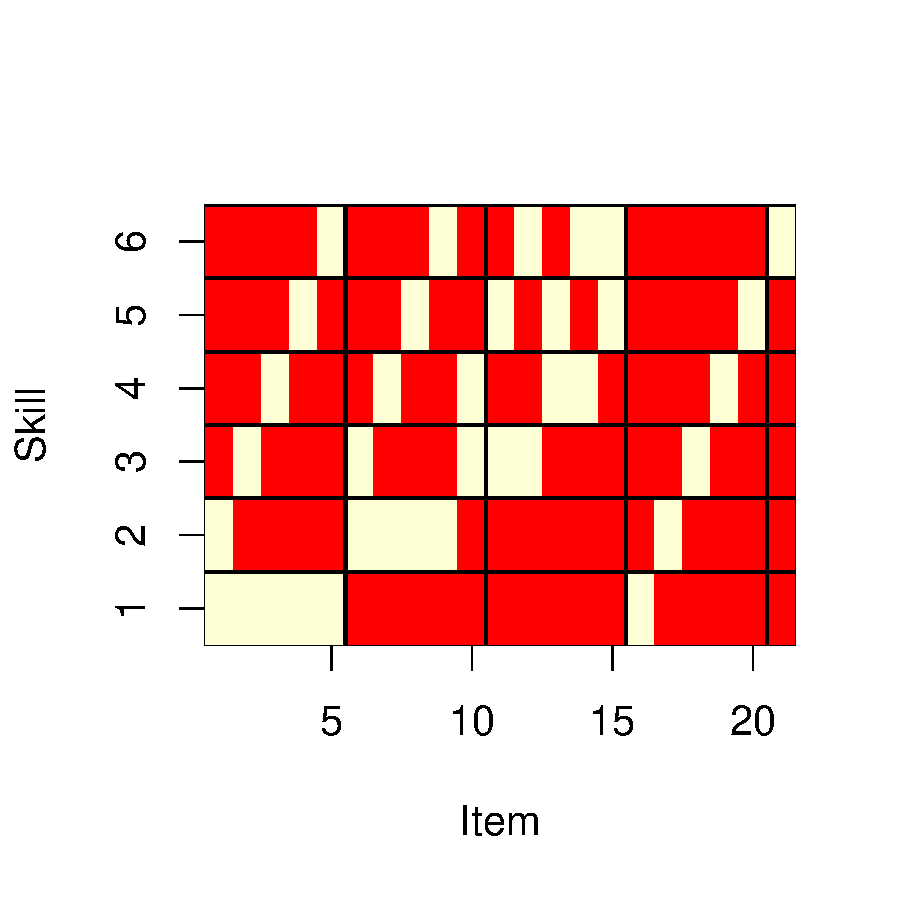
\includegraphics[scale =0.5] {ClustNONnoiseQ}\label{ClustNonnoisyQ}
 }
\centering
\subfigure[Matrix $\hat{\mathbf{Q}}$ with slip and guess factors of 0.2 ($r=0.91$)]{
   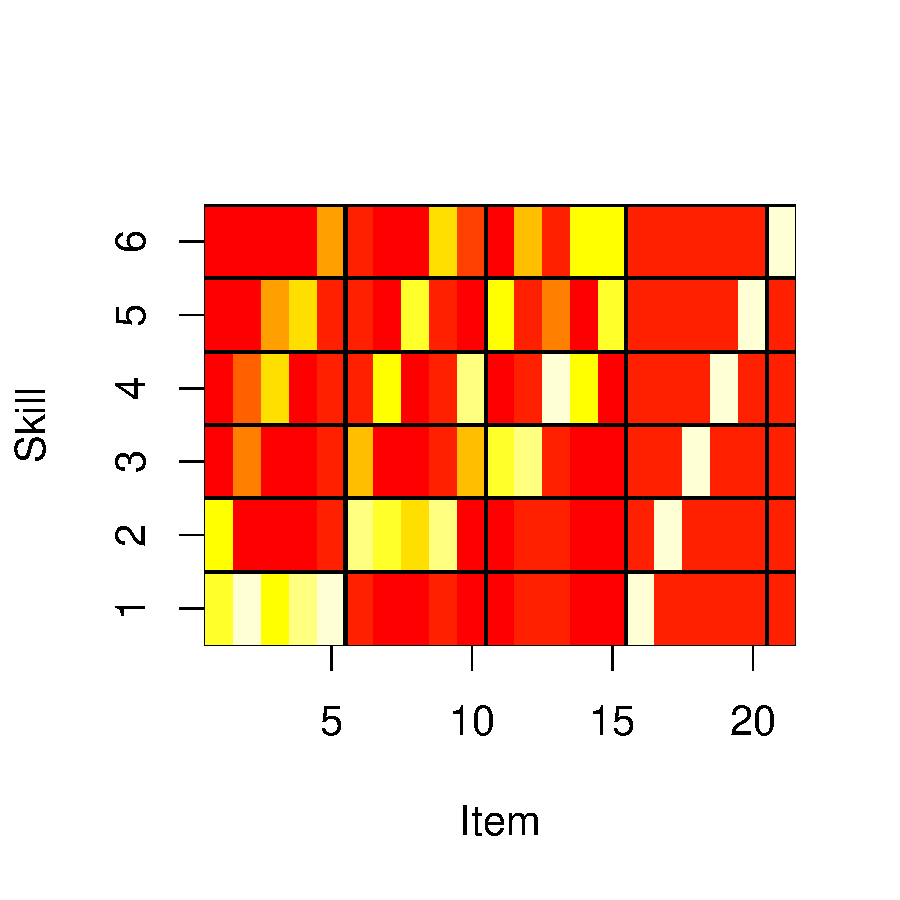
\includegraphics[scale =0.5] {noiseQ}\label{NoisyQ}
 }\quad
 \subfigure[Discretized $\hat{\mathbf{Q}}$ for slip and guess of 0.2 ($r=0.93$).  Three out of 36 skill requirements are incorrectly mapped in this example.]{
   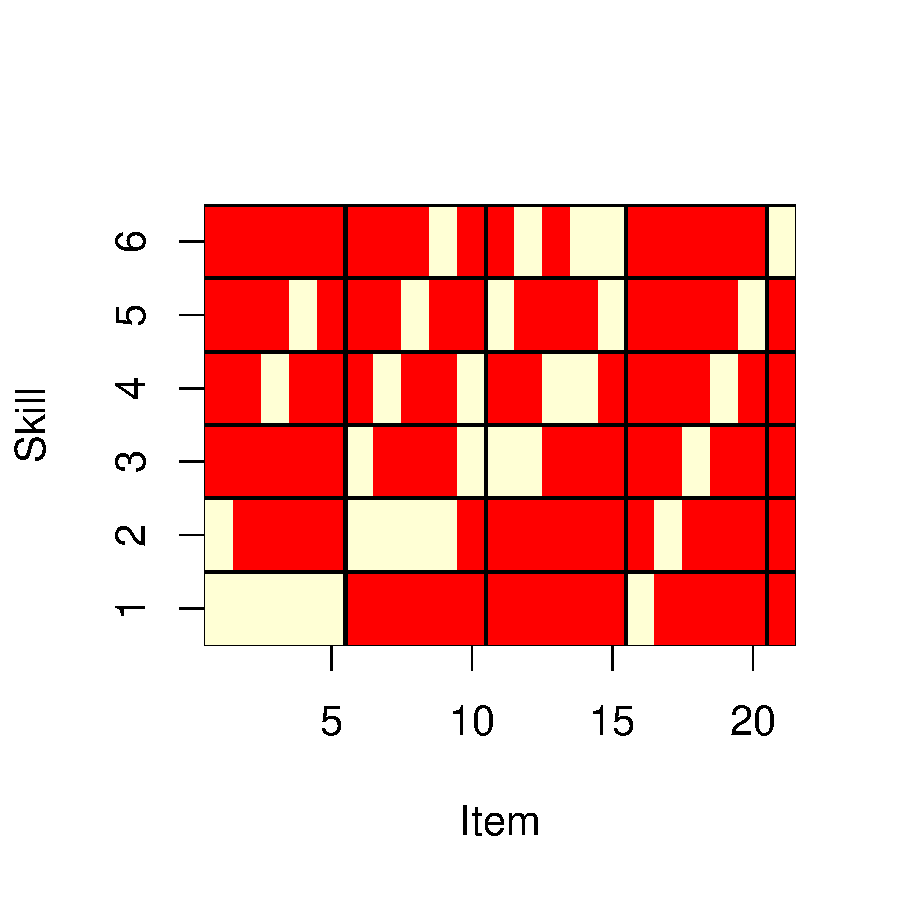
\includegraphics[scale =0.5] {ClustnoiseQ}\label{ClustNoisyQ}
 }
\caption{Visual representations of the original $\mathbf{Q}$ matrix and NMF derived matrices $\hat{\mathbf{Q}}$}
\label{ClusteringResults}
\end{figure}


Figure \ref{NonnoisyQ} shows a heat map of the matrix $\mathbf{Q}$ inferred from an ideal response pattern of 200 simulated examinees. Skill difficulties were set at (0.17, 0.30, 0.43,0.57, 0.70, 0.83) and examinee mean ability and standard deviation respectively at 0 and 0.5. The discretized version of figure \ref{NonnoisyQ}\textquoteright{}s matrix is shown in figure \ref{ClustNonnoisyQ} and it is identical to the underlying matrix $\mathbf{Q}$ in figure \ref{PerfectQ}.

Figure \ref{NonnoisyQ} and \ref{ClustNoisyQ} shows the effect of adding slip and guess parameters of 0.2 for each. The mapping to the underlying matrix $\mathbf{Q}$ degrades as expected, but remains relatively accurate.

Table \ref{tab:wq-comp} reports the results of the quantitative comparison between the $\mathbf{Q}$ matrix and the $\hat{\mathbf{Q}}$ matrix inferred as a function of different slip and guess parameters. These results are based on 10-fold simulations. The mean of the Pearson correlation coefficient (r) between $\mathbf{Q}$ and $\hat{\mathbf{Q}}$ is reported for the discretized version of $\hat{\mathbf{Q}}$ obtained with the clustering algorithm described in previous section. In addition, the error rate as computed by this formula is also provided:

\begin{equation}
  Err = \frac{\sum_{ij} |w_{ij} - q_{ij}| }{2 \cdot \sum_{ij} |q_{ij}| }
\end{equation}
Where $w_{ij}$ and $q_{ij}$ are respectively the $(i,j)$ cells of the matrices $\hat{\mathbf{Q}}$ and $\mathbf{Q}$.  The error rate will be $0$ for a perfectly matched $\mathbf{Q}$ and~$1$ when no cells match.  A value of~$0.5$ indicates that half of the non-zero cells are correctly matched. For the matrix $\mathbf{Q}$, the estimated random error rate is 71\%.

The 0 \textit{slip} and 0 \textit{guess} condition (first line) correspond to figures \ref{NonnoisyQ} and \ref{ClustNonnoisyQ}, whereas the corresponding 0.2--0.2 condition (line~3) correspond to figures\ref{NoisyQ}  and \ref{ClustNoisyQ}.



\newcommand{\ha}[2]{\multicolumn{#1}{c}{\textbf{#2}}}
\newcommand{\hb}[1]{\ha{1}{#1}}
\begin{table}
  \caption{Quantitative comparison between original $\mathbf{Q}$ matrix and NMF derived matrices $\hat{\mathbf{Q}}$.  Results are based on means and standard deviation over 10 simulation runs.}
  \begin{center}
    \newcolumntype{.}{D{.}{.}{-1}}
  \begin{tabular}{cccccc}
    \hline
 \hb{Slip} & \hb{Guess} & \hb{$\overline{r}$} & \hb{sd($\overline{r}$)} & \hb{Err} & \hb{sd(Err)} \\ 
  \hline
0.00 & 0.00 & 1.00 & 0.00 & 0.00 & 0.00 \\ 
0.10 & 0.20 & 0.97 & 0.03 & 0.02 & 0.02 \\ 
0.20 & 0.20 & 0.90 & 0.06 & 0.07 & 0.04 \\ 
0.30 & 0.20 & 0.63 & 0.08 & 0.26 & 0.06 \\ 
0.40 & 0.20 & 0.49 & 0.07 & 0.36 & 0.06 \\ 
  \hline
  \end{tabular}
  \end{center}

\label{tab:wq-comp}
\end{table}

Up to the 0.2--0.2 slip-guess condition, the skill mapping stays relatively close to perfect. On average, approximately only 2 or 3~skills requirements are wrongly assigned out of the 36 skills requirements (7\%) at the 0.2--0.2 condition.  However, the error rate increases substantially at the 0.3--0.2 slip-guess condition, and at the 0.4--0.2 condition, the quality of the match is considerably degraded with an average of 13/36 wrong assignements (36\%).

\subsection{Discussion}

The proposed approach to deriving a conjunctive Q-matrix from simulated data with NMF is successful but, as we can expect, it degrades with the amount of \textit{slips} and \textit{guesses}. If the conjunctive Q-matrix contains one or two items per skill and the noise in the data remains below slip and guess factors of~$0.2$, the approach successfully derives the Q-matrix with very few mismatches of items to skills.  However, once the data has slip and guess factors of~$0.3$ and~$0.2$, then the performance starts to degrade rapidly.

Of course, with a slip factor of~$0.3$ and a guess factor~$0.2$, half the values in the results become inconsistent with the Q-matrix. A substantial degradation is therefore not surprising.  But in this experiment with simulated data, we have a number of advantages that are lost with real data: the number of skills is known in advance, no item has more than two conjunctive skills, skills are independent, and surely other factors will arise to make real data more complex.  Therefore, we can expect that even if real data does not have a 50\% rate of inconsistent results with the examinees' skills mastery profile, other factors might make the induction of the Q-matrix subject to errors of this scale.

\section{Finding the number of latent skills}
\label{EDM2012}

We do not need to identify all the skills behind an item in order to use the item outcome for assessment purpose. As long as we can establish a minimally strong tie from an item to a skill, this is a sufficient condition to use the item in the assessment of that skill. But knowledge that there is a fixed number of determinant factors to predict item outcome is a useful information. For example, if a few number of skills, say 6, are meant to be assessed by a set of 20 questions items, and we find that the underlying number of determinant latent factors behind these items is very different than 6, then it gives us a hint that our 6-skills model may not be congruent with the assessment result.

In an effort towards the goal of finding the skills behind a set of items, we investigate two techniques to determine the number of dominant latent skills. The SVD is a known technique to find latent factors. The singular values represent direct evidence of the strength of latent factors. Application of SVD to finding the number of latent skills is explored. We introduce a second technique based on a wrap- per approach. Linear models with different number of skills are built, and the one that yields the best prediction accuracy through cross validation is considered the most appropriate. The results show that both techniques are effective in identifying the latent factors over synthetic data. An investigation with real data from the fraction algebra domain is also reported. Both the SVD and wrapper methods yield results that have no simple interpretation.


\subsection{SVD-Based method}

SVD is a well known matrix factorization technique that decomposes any matrix, $\mathbf{A}$, into three sub-matrices: 

\begin{equation}
\mathbf{A}=\mathbf{UDV^{T}}\label{eq:SVD}
\end{equation}


where $\mathbf{U}$ and $\mathbf{V}$ are orthonormal matrices and their column vectors respectively represent the eigenvectors of $\mathbf{\mathbf{A}A^{T}}$ and $\mathbf{A^{T}\mathbf{A}}$. $\mathbf{D}$ is a diagonal matrix that contains the singular values. They are the square root of the eigenvalues of the eigenvectors and are sorted in a descending order. Because the singular values represent scaling factors of the unit eigenvectors in equation \ref{eq:SVD}, they are particularly useful in finding latent factors that are dominant in the data. This is demonstrated with simulated data below. The simulated data in this experiment is generated based on the same pattern on the previous section. Again we have all combination of skills for items, at most 2 skills per item and all other factors like slip and guess.


\subsection{Wrapper-Based method}


We introduce a second method to determine the number of dominant skills behind items based on a wrapper approach. In statistical learning, the wrapper approach refers to a general method for selecting the most effective set of variables by measuring the predictive performance of a model with each variables set (see \citep{Guyon2003}). In our context, we assess the predictive performance of linear models embedding different number of latent skills. The model that yields the best predictive performance is deemed to reflect the optimal number of skills.

The wrapper method requires a model that will predict item outcome. A linear model of skills is defined for that purpose on the basis of the equation \ref{eq:1}. This model represents a compensatory interpretation of skills modelling, where each skill contributes additively to the success of an item. The conjunctive model of skills was presented in \ref{eq:6}. To estimate the optimal number of skills, the wrapper model can either correspond to equation\ref{eq:1} or \ref{eq:6}. We will focus our explanations around equation \ref{eq:1}, but they obviously apply to \ref{eq:6} if $\mathbf{R}$ and $\mathbf{S}$ are negated.

This model states that, given estimates of $\mathbf{Q}$ and $\mathbf{S}$, we can predict $\mathbf{R}$. We refer to these estimates as $\hat{\mathbf{Q}}$ and $\hat{\mathbf{S}}$, and to the predictions as $\hat{\mathbf{R}}=\hat{\mathbf{Q}}\hat{\mathbf{S}}$. The goal is therefore to derive estimates of $\hat{\mathbf{Q}}$ and $\hat{\mathbf{S}}$ with different number of skills and measure the residual difference between $\mathbf{R}$ and $\hat{\mathbf{R}}$. 

First, $\hat{\mathbf{Q}}$ is learned from an independent set of training data. Then, $\hat{\mathbf{S}}$ is learned from the test data, and the residuals are computed%
\footnote{Note that computing $\hat{\mathbf{S}}$ from the test data raises the issue of over-fitting, which would keep the accuracy growing with the number of skills regardless of the \textquotedblleft{}real\textquotedblright{} number of skills. However, this issue is mitigated by using independent learning data for $\hat{\mathbf{Q}}$ , without which, we empirically observed, the results would deceive us: in our experiments using both $\mathbf{Q}$ and $\mathbf{S}$ from NMF while increasing the rank of the factorization (number of skills), ends up increasing prediction accuracy even after we reach beyond the \textquotedblleft{}real\textquotedblright{} number of skills. This can reasonably be attributed to over-fitting. %
}.

An estimate of $\hat{\mathbf{Q}}$ is obtained through NMF. Details on applying this technique to the problem of deriving a Q-matrix from data is found in \citep{desmarais2011conditions} and we limit our description to the basic principles and issues here.

The NMF technique requires to choose a rank for the decomposition, which corresponds in our situation to the number of skills (i.e. number of columns of $\mathbf{Q}$ and number of rows of $\mathbf{S}$). Because NMF constrains $\mathbf{Q}$ and $\mathbf{S}$ to non-negative values, their respective interpretation as a Q-matrix and a as student skills assessments is much more natural than other matrix factorization techniques such as Principal Component Analysis, for example. However, multiple solutions exists to this factorization and there are many algorithms that can further constrain solutions, namely to force sparse matrices. Our experiment relies on the R package named NMF and the Brunet algorithm \citep{Gaujoux2010}.

Once $\hat{\mathbf{Q}}$ is obtained, then the values of $\hat{\mathbf{S}}$ can be computed through linear regression. Starting with the overdetermined system of linear equations:

\begin{equation}
\mathbf{R}=\hat{\mathbf{Q}}\hat{\mathbf{S}}\label{eq:Estimation}
\end{equation}


which has the same form as the more familiar $y=\mathbf{X}\beta$ (except that $y$ and $\beta$ are generally vectors instead of matrices), it follows that the linear least squares estimate is given by:

\begin{equation}
\hat{\mathbf{S}}=\left(\hat{\mathbf{Q}}^{T}\hat{\mathbf{Q}}\right)^{-1}\hat{\mathbf{Q}}^{T}\mathbf{R}\label{eq:ShatEstimation}
\end{equation}


Equation \ref{eq:ShatEstimation} represents a linear regression solution which minimizes the residual errors $\left(\left\Vert \mathbf{R}-\hat{\mathbf{Q}}\hat{\mathbf{S}}\right\Vert \right)$.

\subsection{Results of SVD-Based method}


The results of the SVD method are shown in figure \ref{SVD-simul}. The x is the index of the singular value, and the y axis is its actual value. Recall that the singular values of SVD indicate the strength of latent factors.

Three conditions are reported in figure \ref{SVD-simul}. The y values at 1 on the x scale are truncated on the graph to allow a better view of the interesting region of the graph, but the highest value is from the {[}guess=0, slip=0{]} condition and the lowest is for the random condition. The random curve condition can be obtained by simulating random \{0, 1\} values and ensuring that the overall average score of the results matrix reflects the original's data average. In this random condition, the slope from singular value 2 to 21 remains relatively constant, suggesting no specific number of skills. In condition {[}guess=0, slip=0{]}, a sharp drop occurs between singular values of 6 and 7. Then the slope remains relatively constant from values 8 to 21. The largest drop is clearly at value 6 which corresponds to the underlying number of skills. In the third condition {[}guess=0.2, slip=0.1{]}, the largest drop still remains visible between 6 and 7, but not as sharp as for the noiseless condition,
as expected.

In other experiments with various number of skills, not reported here due to space constraints, we observed similar patterns. Another observation is that the random curve intersects with the other two after the number of underlying latent skills (after 6 in figure \ref{SVD-simul}'s experiment).

Therefore, the SVD method does allow for the identification of the number of skills with synthetic data, at least up to the {[}guess=0.2, slip=0.1{]} level.

\begin{figure}
\centering
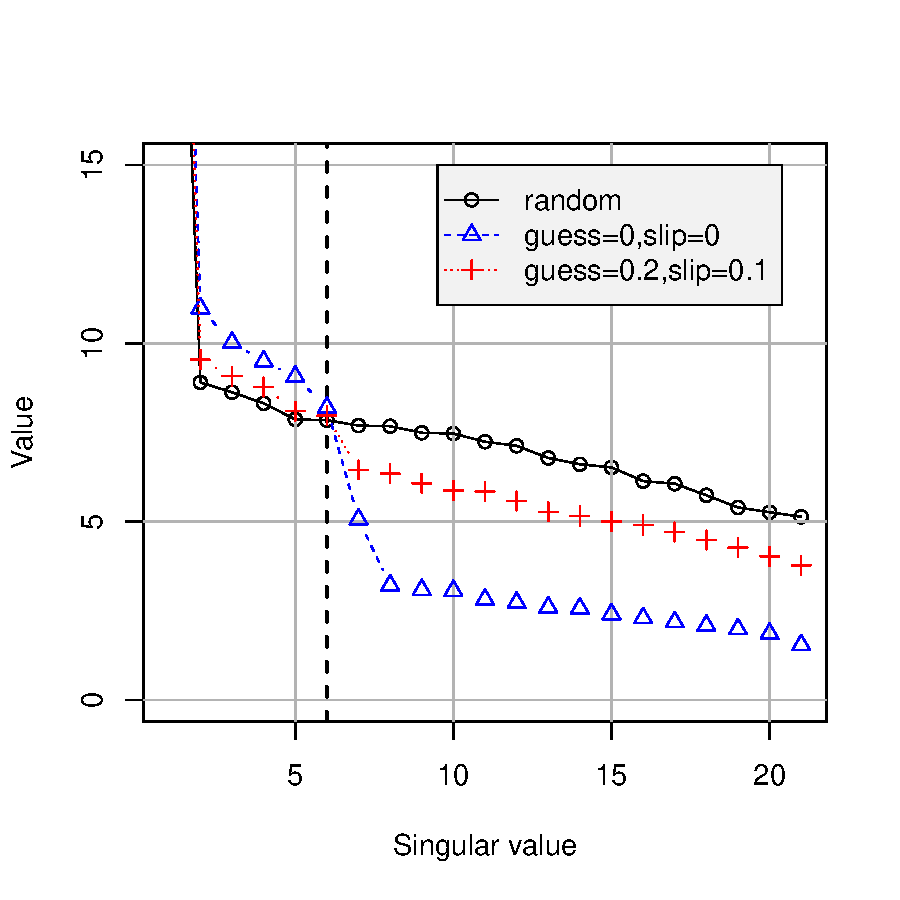
\includegraphics[scale=0.6]{svd-simul}\caption{Singular values of simulated data for a 21 items test. A vertical
dashed line at singular value 6 corresponds to the number of underlying
latent skill factors.}
\label{SVD-simul}

\end{figure}

\subsection{Results of Wrapper-Based method}


We would expect the model with the correct number of skills to perform the best, and models with fewer skills to under- perform because they lack the correct number of latent skills to reflect the response patterns. Models with greater number of skills than required should match the performance of the correct number model, since they have more representative power than needed, but they run higher risk of over- fitting the data and could therefore potentially show lower accuracy in a cross-validation. However, the skills matrix $\hat{\mathbf{S}}$ obtained through equation \ref{eq:ShatEstimation} on the test data could also result in over-fitting that will increase accuracy this time.

Figure \ref{Wrapper} shows the percentage of correct predictions of the models as a function of the number of skills. Given that predictions are \{0,1\}, the percentage can be computed as $\left(\left\Vert \mathbf{R}-\hat{\mathbf{Q}}\hat{\mathbf{S}}\right\Vert \right)/mn$, where m and n are the number of rows and columns of $\mathbf{R}$.

\begin{figure}
\centering

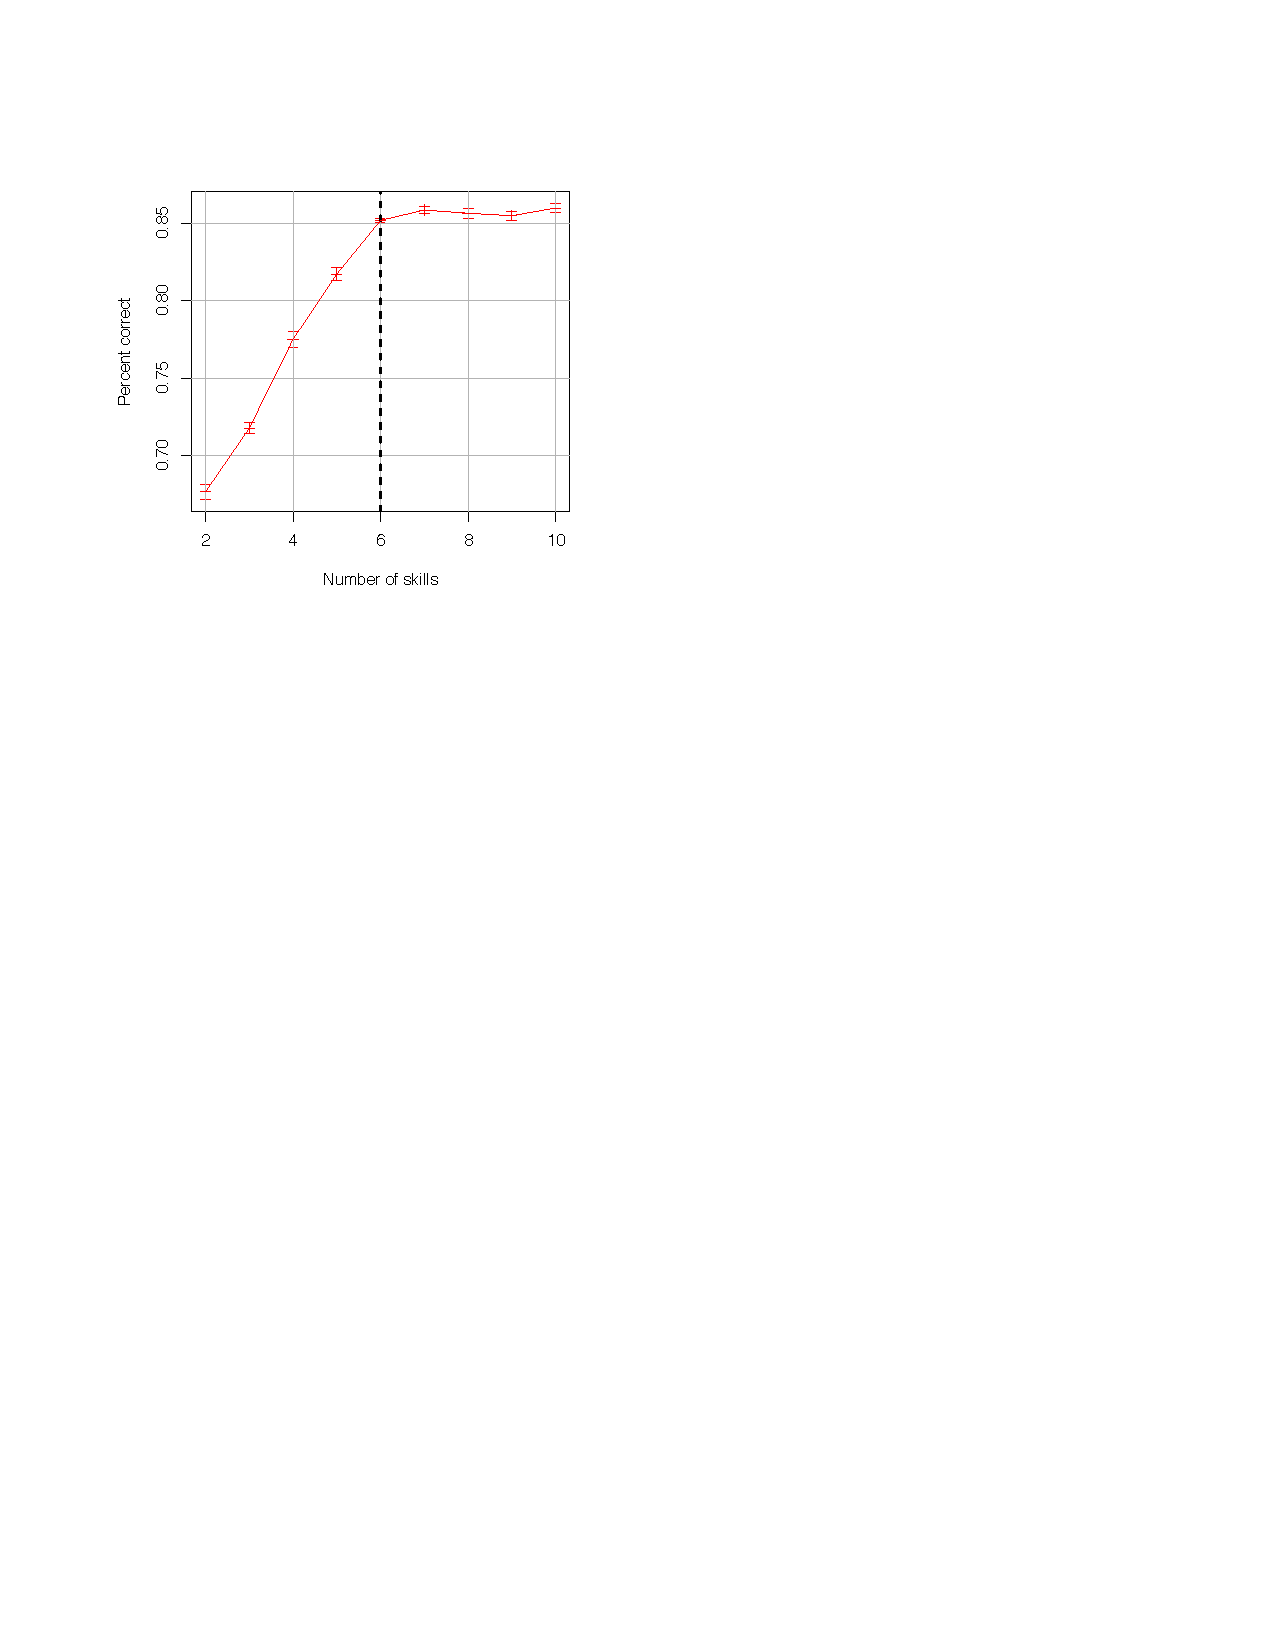
\includegraphics{Wrapper}\caption{Precision of student results predictions from estimated skill matrix
(equation \ref{eq:ShatEstimation}). Error bars are the standard error
of the accuracy curves. Experiment is done with simulated data with
6 skills and slip and guess values of 0.1 and 0.2 respectively.}
\label{Wrapper}
\end{figure}


The results confirm the conjectures above: the predictive accuracy increases until the underlying number of skills is reached, and it almost stabilizes thereafter. Over-fitting of $\hat{\mathbf{S}}$ with the test data is apparently not substantial. It is interesting to note that the accuracy increments of figure \ref{Wrapper} are relatively constant between each skill up to 6. This is also what we would expect since every skill in the underlying Q-matrix has an equivalent weight to all others. We expect that differences in increments indicate differences in the weights of the skills. This could either stem from the structure of the Q-matrix (for e.g., more items can depend on one skill than on another), or on the criticality of the skill over its item outcome.



\subsection{Discussion}
This research showed that Both the SVD and the wrapper methods provide strong cues of the number of underlying skills with simulated student test data.  However, for the Vomlel data set, both methods yield results that are much more ambiguous.  Instead of the 7~skills that were identified by experts over the 17~items set, the SVD method suggests only 2~skills if we rely on the intersection with the random data curve, and no clear number if we look for a change of slope after skill~2.  The wrapper method shows data that is also consistent with 2~skills to the extent that a drop of accuracy is observed at 3~skills, but a rise of accuracy up to 8~skill draws an interpretation closer to the experts' 7 skills set.

An important difference between the SVD and the wrapper methods has to do with the independence of skills.  For SVD, orthogonality of the singular matrices $\mathbf{U}$ and $\mathbf{V}$ in equation~(\ref{eq:1}) forces latent factors to be independent.  NMF does not require latent factors to be independent.  The orthogonality constraint of may limit the application of the SVD method with respect to real skills and might explain some of the difference between the two methods.  The skills from the synthetic data of the first experiment were independent and the Q-matrix had an homogeneous pattern for each skill, and therefore the effect of dependence between skills could not come into play.

Obviously, the study calls for more investigations.  The findings from one set of data from the real world may be highly different from another set. More studies should be conducted to assess the generality of the findings.  Other investigations are called for to find ways to improve these methods and to better understand their limits when faced with real data.  In particular, we need to know at which level of noise from guess and slip factors do the methods break down, and what is the ratio of latent skills to data set size that is critical to avoid over-fitting of the wrapper method.

One improvement that can be brought to the wrapper method is to use a cross validation to derive the skills matrix.  This would require the use of two sets of items, one for testing and one for assessing the student's skills.  This comes at the cost of a greater number of items, but it avoids the problem of over-fitting that leads to accuracy increases.

\section{The refinement of a Q-matrix}
\label{edm2014}

Validating of the expert defined Q-matrix has been the focus of recent developments in the field of educational data mining in recent years \citep{delaTorre2008,chiu2013statistical,barnes2010novel,loye2011validite,Desmarais2013aied}.
In this section we compare three data driven techniques for the validation of skills-to-tasks mappings.  All methods start from a given expert defined Q-matrix, and use optimization techniques to suggest a refined version of the skills-to-task mapping.  
%To validate the different techniques, we inject alterations in the Q-matrix and verify whether the original Q-matrix can be recovered.  Tests are run over both simulated and real data.  The comparison of the techniques over ten data sets shows that, in general, around 1/2 to 2/3 of the alterations can be restored to their original values by the best performer, the ALS matrix factorization method, but the results vary substantially across techniques, and across data sets.


%%%%%%%%%%%%%%%%%%%%%%%%%%%%%%%%%%%%%%%%%%%%%%%%%%%%%%%%%%%%%%%%%%%%%%%%%%%%%
\subsection{Q-matrices validation techniques}

Two techniques for Q-matrix validation surveyed here rely on the DINA and DINO models, whereas one relies on a matrix factorization technique called ALS.  We briefly review each technique below before describing the experiments.


%%%%%%%%%%%%%%%%%%%%%%%%%%%%%%%%%%%%%%%%%%%%%%%%%%%%%%%%%%%%%%%%%%%%%%%%%%%%%
\begin{description}


\item[de~la Torre (2008)] The method defined by de la Torre \citep{delaTorre2008} searches for a Q-matrix that maximizes the difference in the probabilities of a correct response to an item between examinees who possess all the skills required for a correct response to that item and examinees who do not. It first uses the DINA model and an EM algorithm to estimate the slip and guess parameters, after which it can calculate the respective probabilities.  The difference between the two probabilities represents an item discrimination index: the greater the difference between the probability of a correct response given the skills required to the probability given missing skills, the greater the item is discriminant. Therefore we can consider that the method finds a Q-matrix that maximizes item discrimination over all items.

%%%%%%%%%%%%%%%%%%%%%%%%%%%%%%%%%%%%%%%%%%%%%%%%%%%%%%%%%%%%%%%%%%%%%%%%%%%%%

\item[Chiu (2013)] Chiu defines a method that minimizes the residual sum of square (RSS) between the real responses and the ideal responses that follow from a given Q-matrix~\citep{chiu2013statistical}.  The algorithm adjusts the Q-matrix by choosing the item with the worst RSS over to the data, and replaces it with the one has the lowest RSS, and iterates until convergence.

%%%%%%%%%%%%%%%%%%%%%%%%%%%%%%%%%%%%%%%%%%%%%%%%%%%%%%%%%%%%%%%%%%%%%%%%%%%%%
\item[ALS] The  (ALS) method is defined in \citep{Desmarais2013aied}.  Contrary to the other two methods, it does not rely on the DINA model.  Instead, it decomposes the results matrix $\mathbf{R}_{m \times n}$ of~$m$ items by~$n$ students as the inner product two smaller matrices:

\begin{equation}
  \mathbf{{R}} = \mathbf{Q} \, \mathbf{S} \label{eq:nmf}
\end{equation}

where $\mathbf{R}$ is the results matrix ($m$~items by $n$~students),  $\mathbf{Q}$ is the $m$~items by $k$~skillls Q-matrix, and~$\mathbf{S}$ is the mastery matrix of $k$~skills by $n$~students.

\end{description}
%%%%%%%%%%%%%%%%%%%%%%%%%%%%%%%%%%%%%%%%%%%%%%%%%%%%%%%%%%%%%%%%%%%%%%%%%%%%%
\subsection{Methodology and data sets}

\begin{table*}[ht]
\begin{center}
  \caption{\protect\raisebox{0pt}[0pt][6pt]{Data sets}}
  \label{tab:datasets}
  \begin{tabular}{|llccc p{7.75cm} |}
  \hline
  \multicolumn{2}{|c}{\multirow{2}{*}{\textbf{Name}}} & \multicolumn{3}{c}{\bf Number of}  & \multicolumn{1}{c|}{\multirow{2}{*}{\textbf{Description}}}\tabularnewline

  \cline{3-5}
&   & \multicolumn{1}{c@{~~}}{\bf \raisebox{0pt}[12pt][6pt]{Skills}} &
  \multicolumn{1}{@{}c}{\bf Items} &
  \multicolumn{1}{@{~~~}c@{~~~}}{\bf Cases} & \\
  \hline
%\newcounter{exone}\setcounter{exone}{\thei}\refstepcounter{exone}\label{lab:exone} % allows to use ref/label mechanism (although for some reason it has to be above the reference before).
 1. &  Sim. DINA & 3 & 9 & 400 & {Artificial data available from
    the (\texttt{sim.dina}) data set of the CDM package.
  %% Generated with the DINA model.  The slipping errors vary from 0.0 to 0.3. The attributes
  %% are assumed to be mastered with expected probabilities of -0.4 , 0.2, 0.6,
  %% respectively. The correlation of the attributes is 0.3 for attributes 1 and 2, 0.4 for
  %% attributes 1 and 3 and 0.1 for attributes 2 and 3.
} 
\\
  \hline
2. &  Sim. DINO & 3 & 9 & 400 & {Same parameters as No.~1 but using the
    DINO model (\texttt{sim.dino} data set).} \\  
  \hline
3. &  \parbox{2cm}{\raggedright Sim. CDM DINA} & 3 & 12 & 4000 & {Artificial data generated through the
  CDM function \texttt{sim.din}}.\\
  \hline
4. &  Sim. DCM & 3 & 7 & 10000 & {Artificial data from chapter 9 of the book \textit{Diagnostic Measurement} \cite{rupp2010diagnostic}} \\  
  \hline
5. &  ECPE & 3 & 28 & 2922 & {Dataset from \cite{templin2013obtaining} in \cite{torre2009dina}} \\  
  \hline
6. &  Fraction & 8 & 20 & 536 & {Tatsuoka's fraction algebra
problems~\cite{Tatsuoka1984analysis} (see table~1 in~\cite{DeCarlo2011} for a description of the problems
and of the skills). } \\  
  \hline
7. &  Fraction 1 & 5 & 15 & 536 & {15 questions subset of Fraction
    with Q-matrix defined in \cite{torre2009dina}.} \\  
  \hline
8. &  Fraction 2/1 & 3 & 11 & 536 & {11 questions subset of Fraction
    with Q-matrix from \cite{henson2009defining}.} \\  
  \hline
9. &  Fraction 2/2 & 5 & 11 & 536 & {11 questions subset of Fraction
    with Q-matrix from \cite{torre2009dina}.} \\  
  \hline
10. &  Fraction 2/3 & 3 & 11 & 536 & {3 skills version of Fraction~1.} \\  
  \hline
  \end{tabular}
\end{center}
\end{table*}
%% How many changes are suggested by each technique?
%% What about DINO models of the other techniques?

The two first methods, de~la Torre (2008)~\citep{delaTorre2008} and Chiu (2013)~\citep{chiu2013statistical}, have been shown to perform well on artificial data.  On real data, the performance is more blurry.  The ALS factorization method \citep{Desmarais2013aied} has only been tested on one real data set.  But the methodologies used to validate all three techniques in each respective study vary considerably and do not allow for a proper comparison.

To validate and compare the effectiveness of each technique for refining a given Q-matrix, we follow a methodology based on recovering the Q-matrix from a number perturbations: the binary value of a number of cells of the Q-matrix is inverted, and this ``corrupted'' matrix is given as input to each technique.  If the technique recovers the original value of each altered cell, then we consider that it successfully ``refined'' the Q-matrix.

A total of 30 perturbations are randomly injected in each Q-matrices to validate a method's capacity to recover the original matrix.  Note that when a single perturbation is injected, the maximum number of different perturbations is the size of the Q-matrix. Therefore, if is the size of the Q-matrix is smaller than~30, the total number of perturbations is limited to the number of cells in the Q-matrix.

The experiment is repeated for each of the 10~levels of perturbation, and for each of the 10~data sets described later.  This set of experiments is referred to as a single run, and performance measures are averaged over 8~runs.

The measures of performance are the number of \textit{true positives} and \textit{false positives}:
\begin{itemize}
\item \textbf{Mean true positives}: a \textit{true prositive} corresponds to an alteration that was injected in the input, and was correctly switched back to its original value by the method. The measure reported is the number of correctly recovered alterations averaged over the 8~runs. 
\item \textbf{Mean false positive ratio}: a \textit{false positive} corresponds to a changed Q-matrix entry returned by the method, but that was not injected in the input.  Hereto the mean over all perturbation runs is given.
\end{itemize}

For real data, this methodology rests on the assumption that the original matrix is better than the corrupted one, which is not necessarily the case with an expert generated Q-matrix. The expert may be wrong.  However, we have no other means to inform us of the ``real'' Q-matrix and it is reasonable to assume that most of the cells in the Q-matrix are correct.

For synthetic data, this assumption is correct as the Q-matrix is at the source of the generation of the data, but, of course, the model behind the process may not be a reliable reflection of the real cognitive processes involved.  

A total of 10~data sets are used for the validation.  They are freely available from two R~packages: CDM (\url{http://cran.r-project.org/web/packages/CDM/index.html}) \citep{Robitzsch2012} and Chiu (2013) (\url{http://cran.r-project.org/web/packages/NPCD/NPCD.pdf}).  Table~\ref{tab:datasets} contains a short description of each data set.  Note that for the last six data sets, the source data is the same, but different Q-matrices are defined over them and subsets of items are used in the last four: the fraction data set data is used to create four variations through subsets of questions and alternative Q-matrices (Fraction~1, Fraction~2/1, Fraction~2/2, and Fraction~2/3).  The artificial data sets are generated from the well known DINA and DINO models.

For obtaining the results of the de~la Torre (2008) method, we used the R~implementation found in the CDM package~\citep{Robitzsch2012}.  A DINA model and parameter estimation is first built with the default arguments to the \texttt{din} function, and fed to the \texttt{din.validate.qmatrix} function to obtain a refined version of the Q-matrix. For the results of the Chiu (2013) method, the R~NPCD packaged is used (function \texttt{Qrefine}).

\begin{figure*}
\subfigure[{Average recovery rate by number of perturbations (real data)}]{
  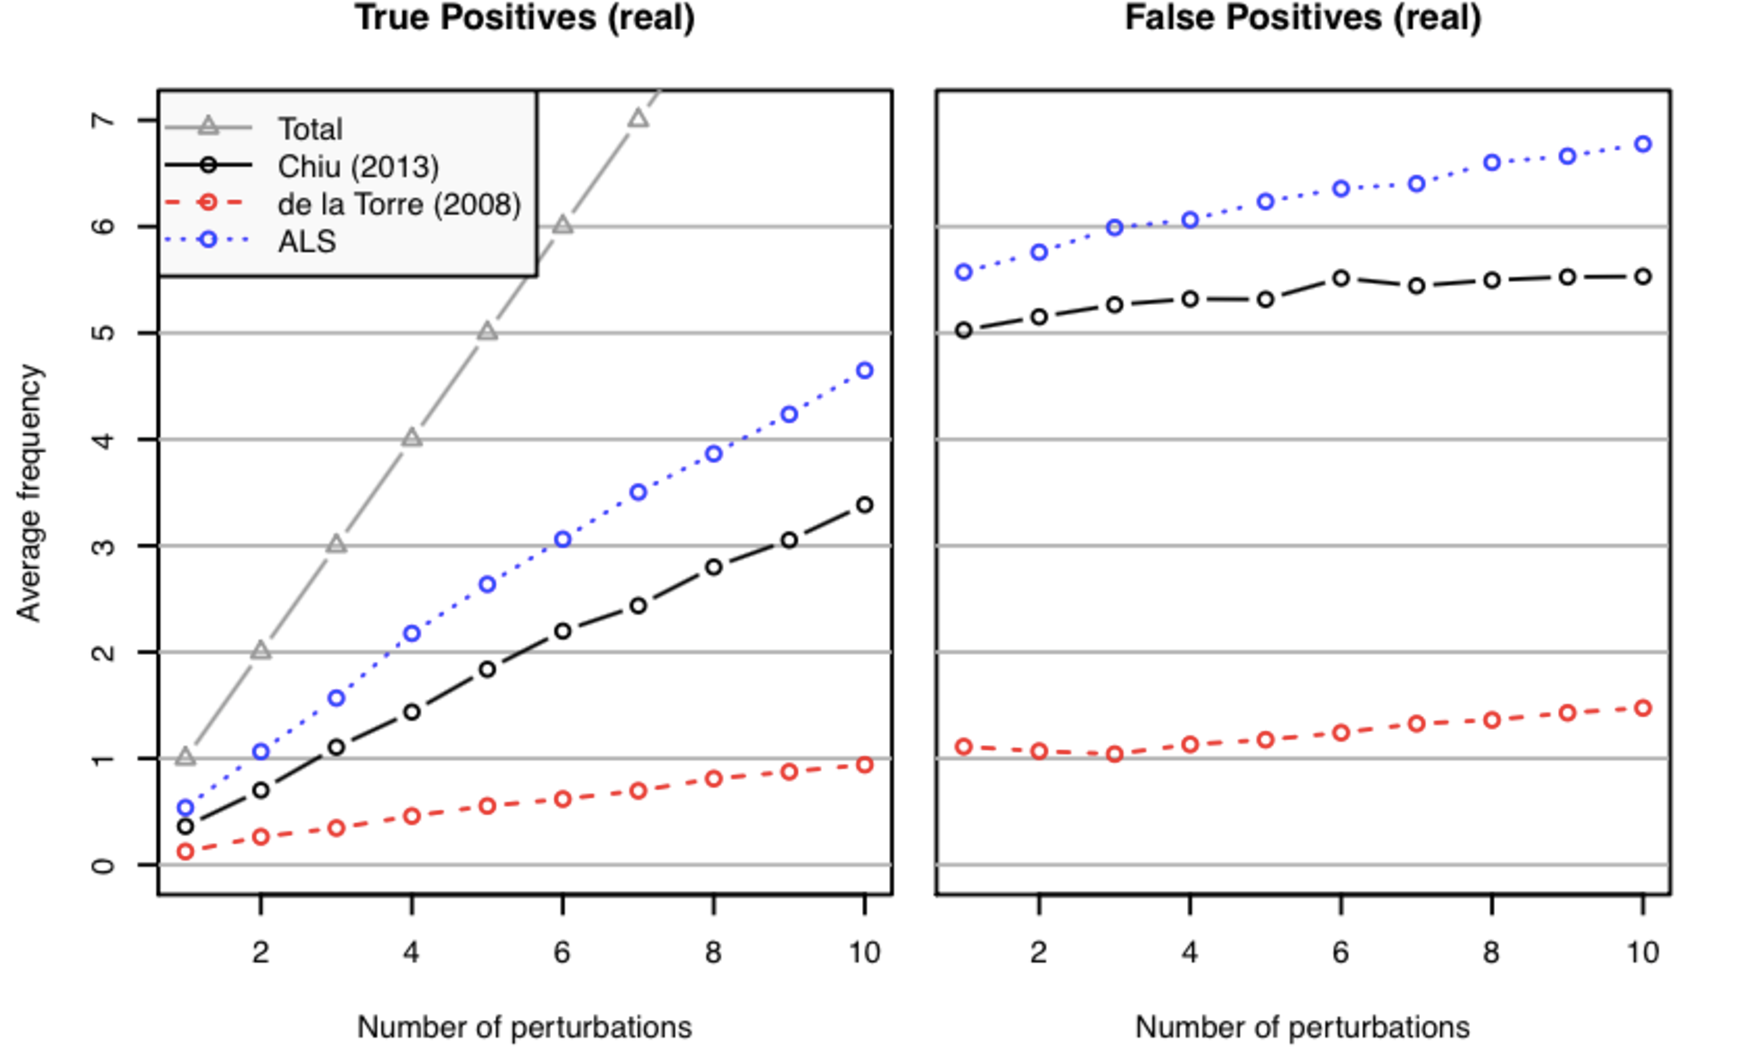
\includegraphics[width=\textwidth]{Images/average-recov.pdf}
  \label{fig:average-recov}
}
\subfigure[{Average recovery rate by number of perturbations (synthetic data)}]{
  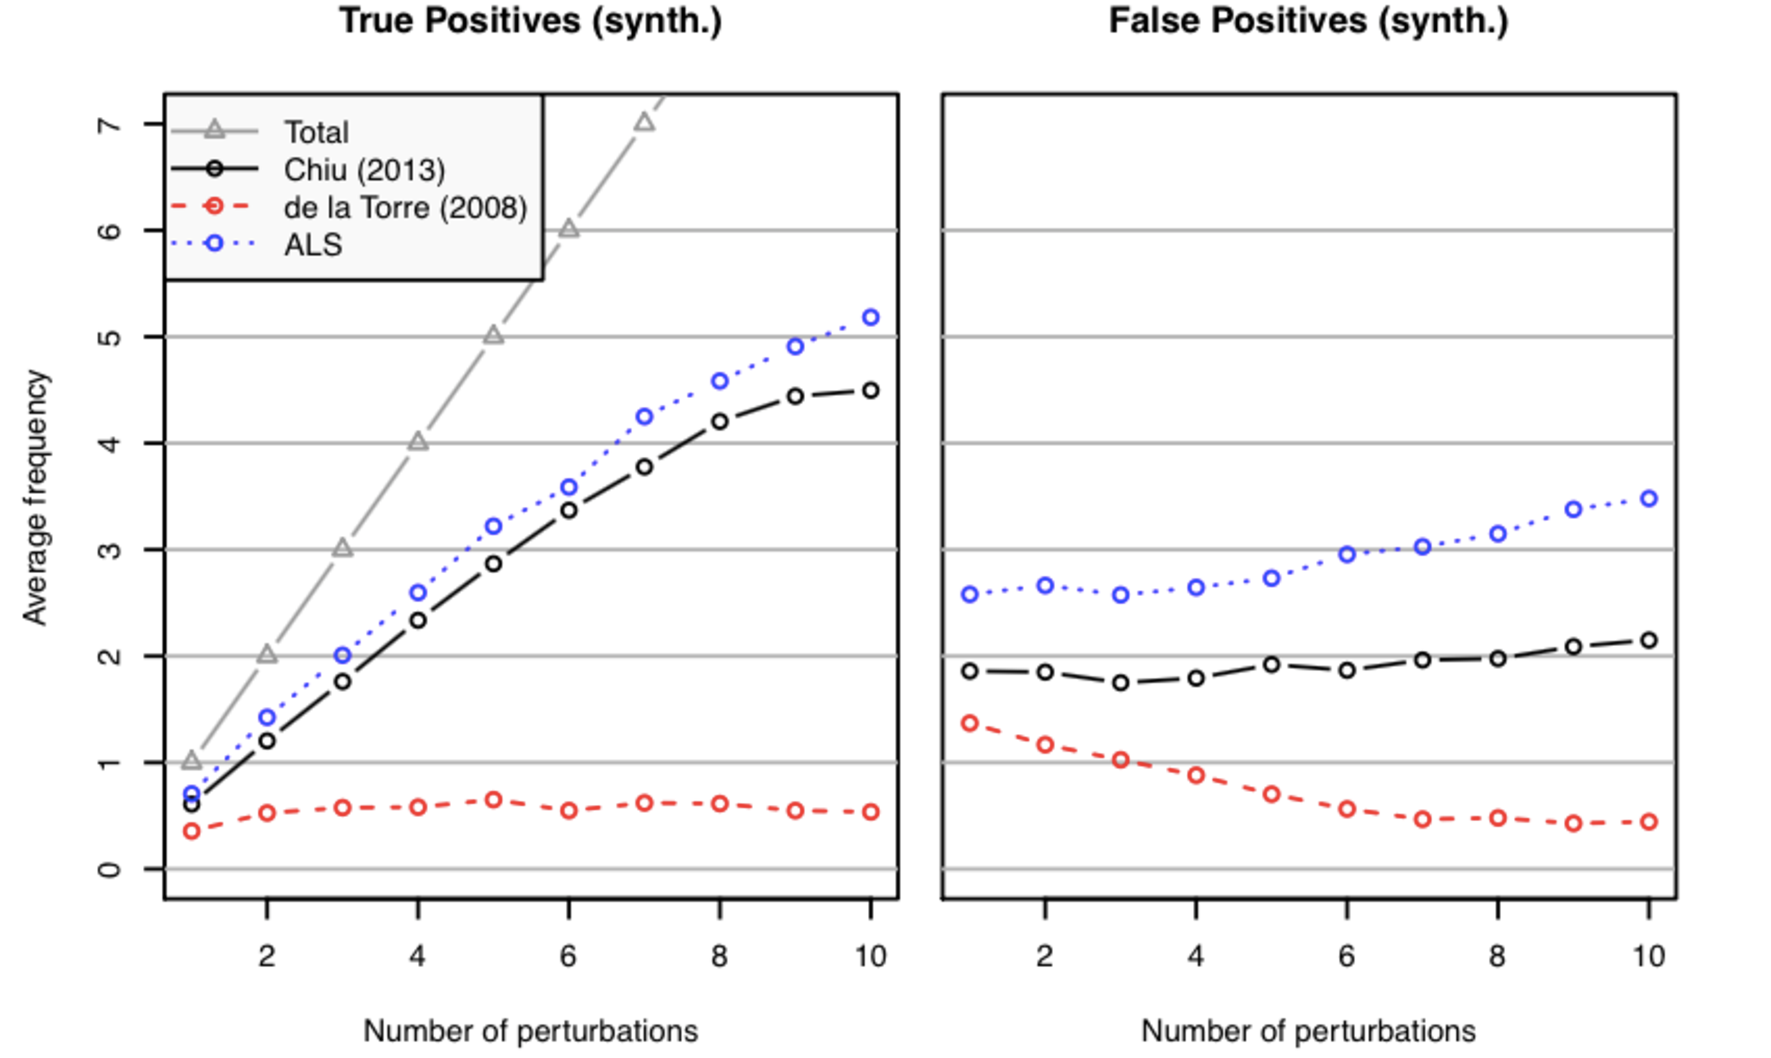
\includegraphics[width=\textwidth]{Images/average-recov-synth.pdf}
  \label{fig:average-recov-synth}
}
  \caption{Average recovery rate by number of perturbations (real and synthetic data). }
\end{figure*}

\begin{sidewaystable} 
  \caption{\protect\raisebox{0pt}[0pt][6pt]{Results by individual data set at 1 and 4 perturbations}}
%  \caption{Single perturbation results}
  \label{tab:details}
\centering
\begin{tabular}{lrrrrrrrrr}
  \hline
  \hline
\raisebox{0pt}[12pt]{~}  & \multicolumn{2}{c}{\textbf{Mean True Positives}} && \multicolumn{2}{c}{\textbf{Mean False Positives}} && \multicolumn{3}{c}{\textbf{TP/FP}}\\
  \cline{2-3} \cline{5-6} \cline{8-10}
\raisebox{0pt}[12pt]{~}   
& \multicolumn{1}{c}{\textbf{ALS}} 
& \multicolumn{1}{c}{\textbf{Chiu (2013)}} 
&
& \multicolumn{1}{c}{\textbf{ALS}} 
& \multicolumn{1}{c}{\textbf{Chiu (2013)}} 
&
& \multicolumn{1}{c}{\textbf{ALS}} 
& \multicolumn{1}{c}{\textbf{Chiu (2013)}} 
& \multicolumn{1}{c}{\textbf{Ratio}} 
\\
  \hline
  \hline
  \multicolumn{2}{l}{\raisebox{0pt}[10pt][6pt]{\textit{Synthetic @ 1 perturbation}}}\\ 
  Sim. DINA & 0.70 (0.00) & 0.55 (0.05) && 2.15 (0.00) & 0.28 (0.05) && 0.33 & 1.95 & 0.3\\ 
  Sim. DINO & 0.48 (0.00) & 0.28 (0.03) && 5.59 (0.00) & 5.30 (0.17) &&  0.09 & 0.05 & 1.8\\ 
  Sim. CDM DINA & 0.93 (0.01) & 1.00 (0.00) && 0.00 (0.00) & 0.00 (0.00) && $\infty$ & $\infty$ & -\\ 
  Sim. DCM & 0.43 (0.00) & 0.14 (0.00) && 0.00 (0.00) & 0.16 (0.02)  && $\infty$ & 0.89 &  $\infty$\\ 
  \hline
  \multicolumn{2}{l}{\raisebox{0pt}[10pt][6pt]{\textit{Real data @ 1 perturbation}}}\\
  ECPE & 0.65 (0.05) & 0.36 (0.03) && 9.81 (0.18) & 17.81 (0.16) && 0.07 & 0.02 & 3.5\\ 
  Fraction & 0.56 (0.07) & 0.46 (0.06) && 5.83 (0.19) & 2.20 (0.27) &&  0.10& 0.21 & 0.5\\ 
  Fraction 1 & 0.65 (0.05) & 0.49 (0.08) && 5.25 (0.17) & 3.14 (0.27) &&  0.12 & 0.16 & 0.8\\ 
  Fraction 2/1 & 0.52 (0.03) & 0.42 (0.03) && 4.56 (0.09) & 5.92 (0.12) &&  0.11 & 0.07 & 1.6\\ 
  Fraction 2/2 & 0.61 (0.09) & 0.41 (0.04) && 4.14 (0.18) & 0.59 (0.12) &&  0.15 & 0.71 & 0.2\\ 
  Fraction 2/3 & 0.36 (0.02) & 0.23 (0.04) && 9.39 (0.07) & 5.37 (0.20) &&  0.04 & 0.04 & 1.0\\ 

  \hline
  \hline
  \multicolumn{2}{l}{\raisebox{0pt}[10pt][6pt]{\textit{Synthetic @ 4 perturbations}}}\\
  Sim. DINA     & 2.55 (0.23) & 1.88 (0.19) && 2.55 (0.34) &  0.95 (0.28) && 1.00 & 1.99 & 0.5\\ 
  Sim. DINO     & 1.69 (0.15) & 1.12 (0.13) && 5.21 (0.19) &  4.43 (0.19) && 0.32 & 0.25 & 1.3\\
  Sim. CDM DINA & 3.57 (0.11) & 4.00 (0.00) && 0.18 (0.07) &  0.00 (0.00) &&19.75 &  Inf & 0.0\\ 
  DCM           & 2.15 (0.25) & 0.53 (0.13) && 1.01 (0.13) &  0.57 (0.12) && 2.13 & 0.94 & 2.3\\ 
  \hline
  \multicolumn{2}{l}{\raisebox{0pt}[10pt][6pt]{\textit{Real data @ 4 perturbations}}}\\
  ECPE          & 2.47 (0.23) & 1.49 (0.21) &&10.59 (0.32) & 17.35 (0.20) && 0.23 & 0.09 & 2.5\\ 
  Fraction      & 2.28 (0.14) & 1.86 (0.15) && 7.93 (0.29) &  2.74 (0.23) && 0.29 & 0.68 & 0.4\\ 
  Fraction 1    & 2.56 (0.08) & 1.95 (0.25) && 5.48 (0.25) &  3.98 (0.23) && 0.47 & 0.49 & 1.9\\ 
  Fraction 2/1  & 2.19 (0.22) & 1.80 (0.20) && 4.92 (0.27) &  5.30 (0.28) && 0.44 & 0.34 & 1.3\\ 
  Fraction 2/2  & 1.90 (0.17) & 1.04 (0.16) && 4.32 (0.35) &  1.91 (0.28) && 0.44 & 0.54 & 0.8\\ 
  Fraction 2/3  & 1.69 (0.15) & 1.41 (0.13) && 8.20 (0.23) &  5.40 (0.24) && 0.21 & 0.26 & 0.8\\ 
  \hline
  \hline
\end{tabular}
\end{sidewaystable} 

%%%%%%%%%%%%%%%%%%%%%%%%%%%%%%%%%%%%%%%%%%%%%%%%%%%%%%%%%%%%%%%%%%%%%%%%%%%%%
\subsection{Results}

The three methods are evaluated over the ten data sets and for ten runs.  Each run is conducted over a set of 30~different random combinations of perturbations, from 1~up to 10~perturbations.  For the 1-perturbation condition, the total number of possible combinations is the size of the Q-matrix itself.

%%%%%%%%%%%%%%%%%%%%%%%%%%%%%%%%%%%%%%%%%%%%%%%%%%%%%%%%%%%%%%%%%%%%%%%%%%%%%
\subsection{Recovery rates by the number perturbation}

Figure~\ref{fig:average-recov} shows the average recovery rate of each method as a function of the number of perturbations.
Recoveries are labeled ``True Positives''~(TP) whereas changes introduced by a method, but which do not correspond to perturbations,
are labeled ``False Positives''~(FP).  The top two graphs show the averages of the 6~real data sets, whereas the bottom graphs show
the averages for the 4~synthetic data sets.  Averages are computed over the 30~perturbations runs (or less if the Q-matrix has
fewer cells).  The ``Total'' line is shown to visually indicate the maximum that can be reached by a TP curve.

The ALS method shows the greatest ability to recover alterations, but at the cost of a higher rate of FP: changes
that do not correspond to perturbations.  It is followed closely by the Chiu (2013) method.  The de~la Torre (2008) method has a very low
rate of recovery (TP) that make it impractical. In general, the ALS and Chiu (2013) methods recover about~2/3 of the
perturbations for synthetic data, and this rate falls to~1/2 for real data with ALS, and about~1/3 for Chiu (2013).  For real
data, the number of FP is around~5 for Chiu (2013) and around~6 for ALS, whereas it is respectively~2 and~3 for
synthetic data. The relative performance of Chiu (2013) with respect to ALS is better for synthetic data and this might be
explained by the fact that the data generation process is directly based on the DINA model.

A common pattern across methods is the relatively stable number of FP as a function of the number of
perturbations.  ALS does show an increase of close to 1~FP between~1 to~10 perturbations, whereas the increase for the Chiu (2013) and
de~la Torre (2008) methods is closer to 1/2 for real data, and even less for synthetic data (in fact it is~$-1$ for de~la Torre (2008)).  As a
result, the rate of TP over FP increases with the number of perturbations.

%%%%%%%%%%%%%%%%%%%%%%%%%%%%%%%%%%%%%%%%%%%%%%%%%%%%%%%%%%%%%%%%%%%%%%%%%%%%%
\subsection{Recovery rates by data set}

The means of TP and FP provide the general trends, but the question remains whether these trends are systematic across each
data set.  To investigate this question we look at the performance details at 1~and at 4~perturbations.  They are reported in
table~\ref{tab:details} for the ALS and Chiu (2013) methods.  The de~la Torre (2008) method is ommitted for brevity and because its
performance is much worst than the other two.

The TP and FP means over the 30 perturbation runs of each individual data set is reported along with
the standard deviation within parenthesis.  We also report the ratio TP/FP. The ``Ratio'' column corresponds to the ALS TP/FP
ratio over the Chiu (2013) TP/FP ratio: a value greater than~1 indicates that the TP/FP ratio is in favor of ALS over Chiu (2013), and
the opposite occurs if the value is less than~1.  Based on this general indicator, we can conclude that the ALS and Chiu (2013) have a
similar performance, but the advantage varies considerably across data sets and can go to either of each method.

Also notable is that the two methods show close to perfect performance at a single perturbation for large simulated data sets
(Sim.~CDM DINA and DCM).  However, at the opposite, they have a weak TP/FP ratio for the ECPE and Fraction~2/3 data sets (from
0.02 to 0.07).  This implies that only between approximately 1~in 50 to 1~in 15 of the proposed Q-matrix changes actually
corresponds to perturbations.  This may prove insufficient for practical purposes, but then again we have to remind ourselves
that not all FP may be considered invalid proposition for changes.  Furthermore on the positive side, the TP/FP ratios at
4~perturbations are more in the range of 1/5 for these same data sets which is a more encouraging.


\subsection{Discussion}

The experiments conducted in section \ref{edm2014} confirm that all methods can recover an altered Q-matrix, as shown in previous work~\cite{delaTorre2008,chiu2013statistical,Desmarais2013aied}. But the comparison of their performance over a number of data sets, and based on a common measure of performance, reveals wide differences.

The ALS matrix factorization technique shows a greater ability to recover alterations than the other two techniques.  For real data, the differences are highly in favor of this method.  Even for data sets made of artificial data generated from the DINA model, with which the two other techniques rely upon for refining the Q-matrix, the ALS factorization performance is comparable or better than the other two techniques.

In addition to revealing the differences of performance among the approaches, the methodology for comparing these techniques is one contribution of this research. Previous work rely on artificial data and parameter fit measures, i.e.\ the difference between an estimated and an the original value of the parameter used to generate the artificial data, as a performance indicator.  However, this approach remains feasible only for models which share the same parameters.  The principle of measuring the proportion of single alterations that are correctly restored is applicable to all models, regardless of their specific parameters.  

This methodology could be enhanced to include sets of more than one alteration, but the number of experimental runs increases exponentially, $(m \times n)^a$ (where~$m \times n$ is the size of the Q-matrix and~$a$ is the number of alterations).  For larger number of alterations, sampling would be needed to contain the growth of runs.

In addition to extending the size of the number of alterations, future work should also extend the comparison to more techniques such as \cite{Liu01102012,loye2011validite}. Finally, we re-iterate the need for open access to the data and the code used in such studies.  This particular study was highly facilitated by the CDM~\cite{Robitzsch2012} and NPCD packages which provided both the code and the data.

\section{Improving matrix factorization techniques of student test data with partial order constraints}
\label{firstcont}

The very first contribution of this thesis was improving the Matrix factorization techniques of student test data with partial order constraints. In particular, we want to address this question: can a \ac{POKS} be used to guide matrix factorization algorithms and lead to faster or better solutions to latent skills modelling?

One avenue to improve over current matrix factorization models is to adapt existing algorithms to the specific nature of the domain data.  In particular, student performance data is known to be constrained by prerequisite relations among skills or knowledge items \cite{falmagne:1990,Doignon1999}.  This constraint can substantially reduce the space of factorization, both for the purpose of assessing student skills and for mapping items to skills.  The objective of this research was to explore how one type of constraints, known as Partial Order Knowledge Structures (POKS), can lead to better factorization techniques for the purposes mentioned.

The very first solution for this improvement is to develop a new factorization algorithm based on the \ac{POKS} constraints. The idea is to change the cost function of the standard \ac{NMF} function. As described in the previous section, standard \ac{NMF} algorithm works based on the cost function in equation \ref{eq:3}. Adding an other value to this cost function can lead to a new equation \ref{eq:7}. 
\begin{equation}
\left\Vert \mathbf{R}-\mathbf{Q}\mathbf{S}\right\Vert ^{2}+\kappa (\mathbf{O}\hat{\mathbf{R}})\label{eq:7}
\end{equation}
where $\kappa$ is a normalizing constant and $\mathbf{O}\hat{\mathbf{R}}$ is the product of the Ordinal incidence matrix gained from POKS algorithm and the expected results matrix obtained from product~$\mathbf{\hat{Q}}\mathbf{\hat{S}}$.

The second term of this formula is a penalizing factor based on the \ac{POKS} constraints. For simplicity we wont explore details of implementation for this part of cost function. 

In order to test the hypothesis we run a simple experiment to see if POKS can give new information which could improve NMF results or not. The methodology is to test NMF, POKS and the combined method with a Bayesian and a Linear generated dataset. The reason for this experiment is to verify if the model behind a dataset can affect the performance of different techniques. Table \ref{Contribution1} shows the result of this experiment. Note that the basic concern of this study is working with noisy data. It was shown that \ac{NMF} perfectly recovers the Q-matrix the with non noisy data, but as some noise like slip or guess was added to the data, the result differs from what was expected \citep{desmarais2011conditions,desmarais2012item}. In this study we want to use another source of knowledge to make an improvement. We should make sure that \ac{POKS} would be correctly derived from both noisy and non-noisy data. In order to generate a noisy data we changed $50\%$ of values for on particular item (say first item) which can represent noise such as slip and guess. The results of experiment showed that NMF could prefectly recover the expected Q-matrix from a linear generated dataset while POKS not even recovered the relations on the noisy item but it presented some false relations between items. On the other hand the estimated Q-matrix from the combined method was not as perfect as the Q-matrix derived from NMF. 


\begin{table}
\center
\caption{Results of running NMF, POKS and combined methods on Linear and Bayesian generated datasets}
\begin{tabular}{|c|c|c|}
\hline
Parameters & Bayesian Generated & Linear Generated\\
\hline
Q-matrix by NMF & Noisy & Perfect\\
\hline
Knowledge Structure by POKS & Perfect & Noisy\\
\hline
Q-matrix by Combined method & Noisy & Noisy\\
\hline

\end{tabular}
\label{Contribution1}
\end{table}

The conclusion that was made out of this hypothesis is: There is a correlation between the underlying model of a dataset and predictive performance of a skills assessment technique. POKS as a Bayesian model can predict the Partial Order parameters of a Bayesian generated dataset better than a linear generated dataset. The reverse is true for factorization techniques on linear generated dataset. 

This experiment showed that combining two different models can not necessarily improve one of them which means that the performance is really depends on the underlying model  of the dataset. This is where we created the second contribution to assess the model fit with comparing the predictive performance of synthetic vs. real dataset.

